\PassOptionsToPackage{unicode=true}{hyperref} % options for packages loaded elsewhere
\PassOptionsToPackage{hyphens}{url}
%
\documentclass[]{article}
\usepackage{lmodern}
\usepackage{amssymb,amsmath}
\usepackage{ifxetex,ifluatex}
\usepackage{fixltx2e} % provides \textsubscript
\ifnum 0\ifxetex 1\fi\ifluatex 1\fi=0 % if pdftex
  \usepackage[T1]{fontenc}
  \usepackage[utf8]{inputenc}
  \usepackage{textcomp} % provides euro and other symbols
\else % if luatex or xelatex
  \usepackage{unicode-math}
  \defaultfontfeatures{Ligatures=TeX,Scale=MatchLowercase}
\fi
% use upquote if available, for straight quotes in verbatim environments
\IfFileExists{upquote.sty}{\usepackage{upquote}}{}
% use microtype if available
\IfFileExists{microtype.sty}{%
\usepackage[]{microtype}
\UseMicrotypeSet[protrusion]{basicmath} % disable protrusion for tt fonts
}{}
\IfFileExists{parskip.sty}{%
\usepackage{parskip}
}{% else
\setlength{\parindent}{0pt}
\setlength{\parskip}{6pt plus 2pt minus 1pt}
}
\usepackage{hyperref}
\hypersetup{
            pdftitle={Extraccion de terminos TFM},
            pdfborder={0 0 0},
            breaklinks=true}
\urlstyle{same}  % don't use monospace font for urls
\usepackage[margin=1in]{geometry}
\usepackage{color}
\usepackage{fancyvrb}
\newcommand{\VerbBar}{|}
\newcommand{\VERB}{\Verb[commandchars=\\\{\}]}
\DefineVerbatimEnvironment{Highlighting}{Verbatim}{commandchars=\\\{\}}
% Add ',fontsize=\small' for more characters per line
\usepackage{framed}
\definecolor{shadecolor}{RGB}{248,248,248}
\newenvironment{Shaded}{\begin{snugshade}}{\end{snugshade}}
\newcommand{\AlertTok}[1]{\textcolor[rgb]{0.94,0.16,0.16}{#1}}
\newcommand{\AnnotationTok}[1]{\textcolor[rgb]{0.56,0.35,0.01}{\textbf{\textit{#1}}}}
\newcommand{\AttributeTok}[1]{\textcolor[rgb]{0.77,0.63,0.00}{#1}}
\newcommand{\BaseNTok}[1]{\textcolor[rgb]{0.00,0.00,0.81}{#1}}
\newcommand{\BuiltInTok}[1]{#1}
\newcommand{\CharTok}[1]{\textcolor[rgb]{0.31,0.60,0.02}{#1}}
\newcommand{\CommentTok}[1]{\textcolor[rgb]{0.56,0.35,0.01}{\textit{#1}}}
\newcommand{\CommentVarTok}[1]{\textcolor[rgb]{0.56,0.35,0.01}{\textbf{\textit{#1}}}}
\newcommand{\ConstantTok}[1]{\textcolor[rgb]{0.00,0.00,0.00}{#1}}
\newcommand{\ControlFlowTok}[1]{\textcolor[rgb]{0.13,0.29,0.53}{\textbf{#1}}}
\newcommand{\DataTypeTok}[1]{\textcolor[rgb]{0.13,0.29,0.53}{#1}}
\newcommand{\DecValTok}[1]{\textcolor[rgb]{0.00,0.00,0.81}{#1}}
\newcommand{\DocumentationTok}[1]{\textcolor[rgb]{0.56,0.35,0.01}{\textbf{\textit{#1}}}}
\newcommand{\ErrorTok}[1]{\textcolor[rgb]{0.64,0.00,0.00}{\textbf{#1}}}
\newcommand{\ExtensionTok}[1]{#1}
\newcommand{\FloatTok}[1]{\textcolor[rgb]{0.00,0.00,0.81}{#1}}
\newcommand{\FunctionTok}[1]{\textcolor[rgb]{0.00,0.00,0.00}{#1}}
\newcommand{\ImportTok}[1]{#1}
\newcommand{\InformationTok}[1]{\textcolor[rgb]{0.56,0.35,0.01}{\textbf{\textit{#1}}}}
\newcommand{\KeywordTok}[1]{\textcolor[rgb]{0.13,0.29,0.53}{\textbf{#1}}}
\newcommand{\NormalTok}[1]{#1}
\newcommand{\OperatorTok}[1]{\textcolor[rgb]{0.81,0.36,0.00}{\textbf{#1}}}
\newcommand{\OtherTok}[1]{\textcolor[rgb]{0.56,0.35,0.01}{#1}}
\newcommand{\PreprocessorTok}[1]{\textcolor[rgb]{0.56,0.35,0.01}{\textit{#1}}}
\newcommand{\RegionMarkerTok}[1]{#1}
\newcommand{\SpecialCharTok}[1]{\textcolor[rgb]{0.00,0.00,0.00}{#1}}
\newcommand{\SpecialStringTok}[1]{\textcolor[rgb]{0.31,0.60,0.02}{#1}}
\newcommand{\StringTok}[1]{\textcolor[rgb]{0.31,0.60,0.02}{#1}}
\newcommand{\VariableTok}[1]{\textcolor[rgb]{0.00,0.00,0.00}{#1}}
\newcommand{\VerbatimStringTok}[1]{\textcolor[rgb]{0.31,0.60,0.02}{#1}}
\newcommand{\WarningTok}[1]{\textcolor[rgb]{0.56,0.35,0.01}{\textbf{\textit{#1}}}}
\usepackage{graphicx,grffile}
\makeatletter
\def\maxwidth{\ifdim\Gin@nat@width>\linewidth\linewidth\else\Gin@nat@width\fi}
\def\maxheight{\ifdim\Gin@nat@height>\textheight\textheight\else\Gin@nat@height\fi}
\makeatother
% Scale images if necessary, so that they will not overflow the page
% margins by default, and it is still possible to overwrite the defaults
% using explicit options in \includegraphics[width, height, ...]{}
\setkeys{Gin}{width=\maxwidth,height=\maxheight,keepaspectratio}
\setlength{\emergencystretch}{3em}  % prevent overfull lines
\providecommand{\tightlist}{%
  \setlength{\itemsep}{0pt}\setlength{\parskip}{0pt}}
\setcounter{secnumdepth}{0}
% Redefines (sub)paragraphs to behave more like sections
\ifx\paragraph\undefined\else
\let\oldparagraph\paragraph
\renewcommand{\paragraph}[1]{\oldparagraph{#1}\mbox{}}
\fi
\ifx\subparagraph\undefined\else
\let\oldsubparagraph\subparagraph
\renewcommand{\subparagraph}[1]{\oldsubparagraph{#1}\mbox{}}
\fi

% set default figure placement to htbp
\makeatletter
\def\fps@figure{htbp}
\makeatother


\title{Extraccion de terminos TFM}
\author{}
\date{\vspace{-2.5em}}

\begin{document}
\maketitle

This is an \href{http://rmarkdown.rstudio.com}{R Markdown} Notebook.
When you execute code within the notebook, the results appear beneath
the code.

Try executing this chunk by clicking the \emph{Run} button within the
chunk or by placing your cursor inside it and pressing
\emph{Ctrl+Shift+Enter}.

Add a new chunk by clicking the \emph{Insert Chunk} button on the
toolbar or by pressing \emph{Ctrl+Alt+I}.

When you save the notebook, an HTML file containing the code and output
will be saved alongside it (click the \emph{Preview} button or press
\emph{Ctrl+Shift+K} to preview the HTML file).

The preview shows you a rendered HTML copy of the contents of the
editor. Consequently, unlike \emph{Knit}, \emph{Preview} does not run
any R code chunks. Instead, the output of the chunk when it was last run
in the editor is displayed.

Leemos los documentos.

\begin{verbatim}
## [1] "Se han leido los documentos del corpus con éxito"
\end{verbatim}

Creamos el corpus de quanteda

\begin{Shaded}
\begin{Highlighting}[]
\KeywordTok{library}\NormalTok{(quanteda)}
\end{Highlighting}
\end{Shaded}

\begin{verbatim}
## Package version: 1.5.2
\end{verbatim}

\begin{verbatim}
## Parallel computing: 2 of 16 threads used.
\end{verbatim}

\begin{verbatim}
## See https://quanteda.io for tutorials and examples.
\end{verbatim}

\begin{verbatim}
## 
## Attaching package: 'quanteda'
\end{verbatim}

\begin{verbatim}
## The following object is masked from 'package:utils':
## 
##     View
\end{verbatim}

\begin{Shaded}
\begin{Highlighting}[]
\CommentTok{# create quanteda corpus}
\KeywordTok{quanteda_options}\NormalTok{(}\DataTypeTok{threads =}\NormalTok{ hilos)}
\NormalTok{quancorpusDocs <-}\StringTok{ }\KeywordTok{corpus}\NormalTok{(docs)}

\CommentTok{#Obtenemos un resumen del corpus que hemops creado}
\NormalTok{summ <-}\StringTok{ }\KeywordTok{summary}\NormalTok{(quancorpusDocs,    }\CommentTok{#Esto tarda unos segundos. Types es el num de tokens Únicos.}
                \DataTypeTok{n =} \KeywordTok{nrow}\NormalTok{(docs))    }\CommentTok{#Por defecto son 100}
\KeywordTok{sum}\NormalTok{(summ}\OperatorTok{$}\NormalTok{Sentences)}
\end{Highlighting}
\end{Shaded}

\begin{verbatim}
## [1] 18588
\end{verbatim}

\begin{Shaded}
\begin{Highlighting}[]
\KeywordTok{sum}\NormalTok{(summ}\OperatorTok{$}\NormalTok{Tokens)}
\end{Highlighting}
\end{Shaded}

\begin{verbatim}
## [1] 523006
\end{verbatim}

\begin{Shaded}
\begin{Highlighting}[]
\CommentTok{#Puedo sacar los textos }
\NormalTok{tDocs <-}\StringTok{ }\KeywordTok{texts}\NormalTok{(quancorpusDocs) }\CommentTok{#No tarda nada. }
                       \CommentTok{#Un vector nombrado (cada elemento tiene el nombre del doc). }
                       \CommentTok{#Cada elemento es una cadena con el texto del doc.}
\end{Highlighting}
\end{Shaded}

Descargamos el modelo udpipe de Google y extraemos los terminos.

\begin{Shaded}
\begin{Highlighting}[]
\KeywordTok{library}\NormalTok{(udpipe)}
\KeywordTok{library}\NormalTok{(tictoc)}

\NormalTok{model <-}\StringTok{ }\KeywordTok{udpipe_download_model}\NormalTok{(}\DataTypeTok{language =} \StringTok{"spanish"}\NormalTok{)}
\end{Highlighting}
\end{Shaded}

\begin{verbatim}
## Downloading udpipe model from https://raw.githubusercontent.com/jwijffels/udpipe.models.ud.2.4/master/inst/udpipe-ud-2.4-190531/spanish-gsd-ud-2.4-190531.udpipe to /Users/pedrohv/TFM/spanish-gsd-ud-2.4-190531.udpipe
\end{verbatim}

\begin{verbatim}
## Visit https://github.com/jwijffels/udpipe.models.ud.2.4 for model license details
\end{verbatim}

\begin{Shaded}
\begin{Highlighting}[]
\CommentTok{#udmodel_spanish_gsd <- udpipe_load_model(file = 'spanish-gsd-ud-2.4-190531.udpipe')}

\NormalTok{path <-}\StringTok{ }\NormalTok{model}\OperatorTok{$}\NormalTok{file_model}

\KeywordTok{tic}\NormalTok{()}
\NormalTok{x <-}\StringTok{ }\KeywordTok{udpipe}\NormalTok{(tDocs, path, }\DataTypeTok{parallel.cores =}\NormalTok{ hilos)}
\KeywordTok{toc}\NormalTok{()}
\end{Highlighting}
\end{Shaded}

\begin{verbatim}
## 113.623 sec elapsed
\end{verbatim}

\begin{Shaded}
\begin{Highlighting}[]
\KeywordTok{saveRDS}\NormalTok{(x, }\DataTypeTok{file =} \StringTok{"termExtraction/udpipeEspañol1.rds"}\NormalTok{)}
\CommentTok{#x <- readRDS(file = "airbus.rds")}
\end{Highlighting}
\end{Shaded}

\begin{Shaded}
\begin{Highlighting}[]
\KeywordTok{library}\NormalTok{(lattice)}

\CommentTok{#Plotting Part-of-speech tags from the given text}

\NormalTok{stats <-}\StringTok{ }\KeywordTok{txt_freq}\NormalTok{(x}\OperatorTok{$}\NormalTok{upos) }\CommentTok{#upos = universal part of speech}
\NormalTok{stats}\OperatorTok{$}\NormalTok{key <-}\StringTok{ }\KeywordTok{factor}\NormalTok{(stats}\OperatorTok{$}\NormalTok{key, }\DataTypeTok{levels =} \KeywordTok{rev}\NormalTok{(stats}\OperatorTok{$}\NormalTok{key))}
\KeywordTok{barchart}\NormalTok{(key }\OperatorTok{~}\StringTok{ }\NormalTok{freq, }\DataTypeTok{data =}\NormalTok{ stats, }\DataTypeTok{col =} \StringTok{"yellow"}\NormalTok{, }
         \DataTypeTok{main =} \StringTok{"UPOS (Universal Parts of Speech)}\CharTok{\textbackslash{}n}\StringTok{ frequency of occurrence"}\NormalTok{, }
         \DataTypeTok{xlab =} \StringTok{"Freq"}\NormalTok{)}
\end{Highlighting}
\end{Shaded}

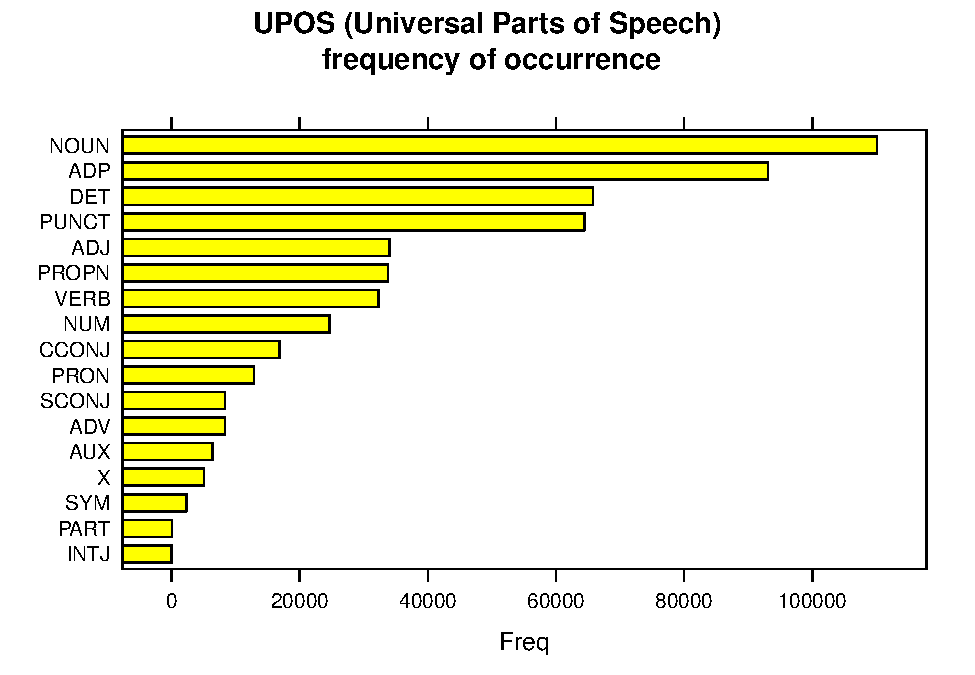
\includegraphics{TFM_files/figure-latex/unnamed-chunk-4-1.pdf}

\begin{Shaded}
\begin{Highlighting}[]
\NormalTok{stats <-}\StringTok{ }\KeywordTok{subset}\NormalTok{(x, upos }\OperatorTok\StringTok{ "NOUN"}\NormalTok{)}
\NormalTok{stats <-}\StringTok{ }\KeywordTok{txt_freq}\NormalTok{(}\DataTypeTok{x =}\NormalTok{ stats}\OperatorTok{$}\NormalTok{lemma)}
\NormalTok{stats}\OperatorTok{$}\NormalTok{key <-}\StringTok{ }\KeywordTok{factor}\NormalTok{(stats}\OperatorTok{$}\NormalTok{key, }\DataTypeTok{levels =} \KeywordTok{rev}\NormalTok{(stats}\OperatorTok{$}\NormalTok{key))}
\KeywordTok{barchart}\NormalTok{(key }\OperatorTok{~}\StringTok{ }\NormalTok{freq, }\DataTypeTok{data =} \KeywordTok{head}\NormalTok{(stats, }\DecValTok{30}\NormalTok{), }\DataTypeTok{col =} \StringTok{"cadetblue"}\NormalTok{, }\DataTypeTok{main =} \StringTok{"Most occurring nouns"}\NormalTok{, }\DataTypeTok{xlab =} \StringTok{"Freq"}\NormalTok{)}
\end{Highlighting}
\end{Shaded}

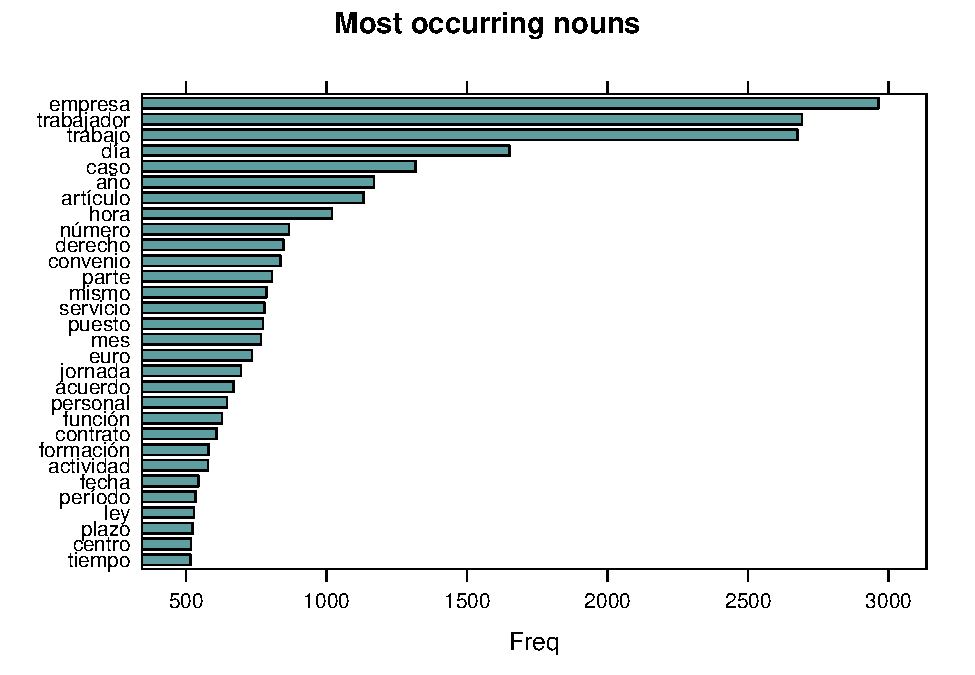
\includegraphics{TFM_files/figure-latex/unnamed-chunk-5-1.pdf}

\begin{Shaded}
\begin{Highlighting}[]
\NormalTok{stats <-}\StringTok{ }\KeywordTok{subset}\NormalTok{(x, upos }\OperatorTok\StringTok{ }\KeywordTok{c}\NormalTok{(}\StringTok{"VERB"}\NormalTok{)) }
\NormalTok{stats <-}\StringTok{ }\KeywordTok{txt_freq}\NormalTok{(stats}\OperatorTok{$}\NormalTok{token)}\CommentTok{# también puedo poner lemma si quiero ver el verbo en infinitivo}
\NormalTok{stats}\OperatorTok{$}\NormalTok{key <-}\StringTok{ }\KeywordTok{factor}\NormalTok{(stats}\OperatorTok{$}\NormalTok{key, }\DataTypeTok{levels =} \KeywordTok{rev}\NormalTok{(stats}\OperatorTok{$}\NormalTok{key))}
\KeywordTok{barchart}\NormalTok{(key }\OperatorTok{~}\StringTok{ }\NormalTok{freq, }\DataTypeTok{data =} \KeywordTok{head}\NormalTok{(stats, }\DecValTok{20}\NormalTok{), }\DataTypeTok{col =} \StringTok{"gold"}\NormalTok{, }
         \DataTypeTok{main =} \StringTok{"Most occurring Verbs"}\NormalTok{, }\DataTypeTok{xlab =} \StringTok{"Freq"}\NormalTok{)}
\end{Highlighting}
\end{Shaded}

\begin{verbatim}
## Warning in grid.Call(C_textBounds, as.graphicsAnnot(x$label), x$x, x$y, : font
## width unknown for character 0x0
\end{verbatim}

\begin{verbatim}
## Warning in grid.Call(C_textBounds, as.graphicsAnnot(x$label), x$x, x$y, : font
## width unknown for character 0x7f
\end{verbatim}

\begin{verbatim}
## Warning in grid.Call(C_textBounds, as.graphicsAnnot(x$label), x$x, x$y, : font
## width unknown for character 0x0
\end{verbatim}

\begin{verbatim}
## Warning in grid.Call(C_textBounds, as.graphicsAnnot(x$label), x$x, x$y, : font
## width unknown for character 0x7f
\end{verbatim}

\begin{verbatim}
## Warning in grid.Call(C_textBounds, as.graphicsAnnot(x$label), x$x, x$y, : font
## width unknown for character 0xa0
\end{verbatim}

\begin{verbatim}
## Warning in grid.Call(C_textBounds, as.graphicsAnnot(x$label), x$x, x$y, : font
## width unknown for character 0x7f
\end{verbatim}

\begin{verbatim}
## Warning in grid.Call(C_textBounds, as.graphicsAnnot(x$label), x$x, x$y, : font
## width unknown for character 0xa0
\end{verbatim}

\begin{verbatim}
## Warning in grid.Call(C_textBounds, as.graphicsAnnot(x$label), x$x, x$y, : font
## width unknown for character 0x7f
\end{verbatim}

\begin{verbatim}
## Warning in grid.Call.graphics(C_text, as.graphicsAnnot(x$label), x$x, x$y, :
## font width unknown for character 0x90
\end{verbatim}

\begin{verbatim}
## Warning in grid.Call.graphics(C_text, as.graphicsAnnot(x$label), x$x, x$y, :
## font width unknown for character 0x7f
\end{verbatim}

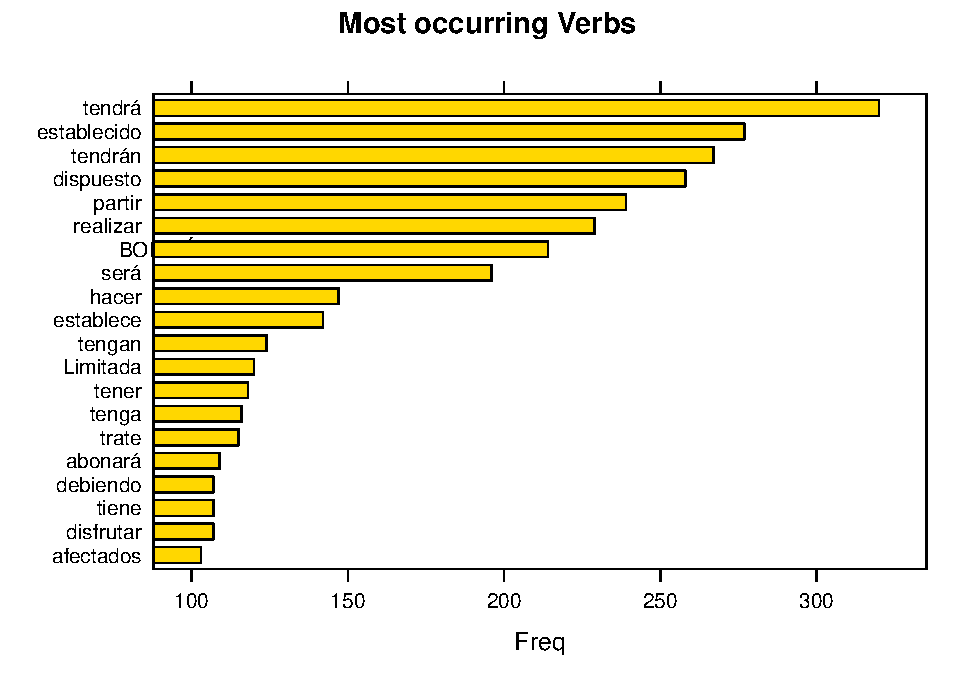
\includegraphics{TFM_files/figure-latex/unnamed-chunk-6-1.pdf}

\begin{Shaded}
\begin{Highlighting}[]
\NormalTok{stats <-}\StringTok{ }\KeywordTok{subset}\NormalTok{(x, upos }\OperatorTok\StringTok{ }\KeywordTok{c}\NormalTok{(}\StringTok{"VERB"}\NormalTok{)) }
\NormalTok{stats <-}\StringTok{ }\KeywordTok{txt_freq}\NormalTok{(stats}\OperatorTok{$}\NormalTok{lemma)}\CommentTok{# el lemma para el verbo en infinitivo}
\NormalTok{stats}\OperatorTok{$}\NormalTok{key <-}\StringTok{ }\KeywordTok{factor}\NormalTok{(stats}\OperatorTok{$}\NormalTok{key, }\DataTypeTok{levels =} \KeywordTok{rev}\NormalTok{(stats}\OperatorTok{$}\NormalTok{key))}
\KeywordTok{barchart}\NormalTok{(key }\OperatorTok{~}\StringTok{ }\NormalTok{freq, }\DataTypeTok{data =} \KeywordTok{head}\NormalTok{(stats, }\DecValTok{20}\NormalTok{), }\DataTypeTok{col =} \StringTok{"gold"}\NormalTok{, }
         \DataTypeTok{main =} \StringTok{"Most occurring Verbs (lemma)"}\NormalTok{, }\DataTypeTok{xlab =} \StringTok{"Freq"}\NormalTok{)}
\end{Highlighting}
\end{Shaded}

\begin{verbatim}
## Warning in grid.Call(C_textBounds, as.graphicsAnnot(x$label), x$x, x$y, : font
## width unknown for character 0x0
\end{verbatim}

\begin{verbatim}
## Warning in grid.Call(C_textBounds, as.graphicsAnnot(x$label), x$x, x$y, : font
## width unknown for character 0x7f
\end{verbatim}

\begin{verbatim}
## Warning in grid.Call(C_textBounds, as.graphicsAnnot(x$label), x$x, x$y, : font
## width unknown for character 0x0
\end{verbatim}

\begin{verbatim}
## Warning in grid.Call(C_textBounds, as.graphicsAnnot(x$label), x$x, x$y, : font
## width unknown for character 0x7f
\end{verbatim}

\begin{verbatim}
## Warning in grid.Call(C_textBounds, as.graphicsAnnot(x$label), x$x, x$y, : font
## width unknown for character 0xa0
\end{verbatim}

\begin{verbatim}
## Warning in grid.Call(C_textBounds, as.graphicsAnnot(x$label), x$x, x$y, : font
## width unknown for character 0x7f
\end{verbatim}

\begin{verbatim}
## Warning in grid.Call(C_textBounds, as.graphicsAnnot(x$label), x$x, x$y, : font
## width unknown for character 0xa0
\end{verbatim}

\begin{verbatim}
## Warning in grid.Call(C_textBounds, as.graphicsAnnot(x$label), x$x, x$y, : font
## width unknown for character 0x7f
\end{verbatim}

\begin{verbatim}
## Warning in grid.Call.graphics(C_text, as.graphicsAnnot(x$label), x$x, x$y, :
## font width unknown for character 0x90
\end{verbatim}

\begin{verbatim}
## Warning in grid.Call.graphics(C_text, as.graphicsAnnot(x$label), x$x, x$y, :
## font width unknown for character 0x7f
\end{verbatim}

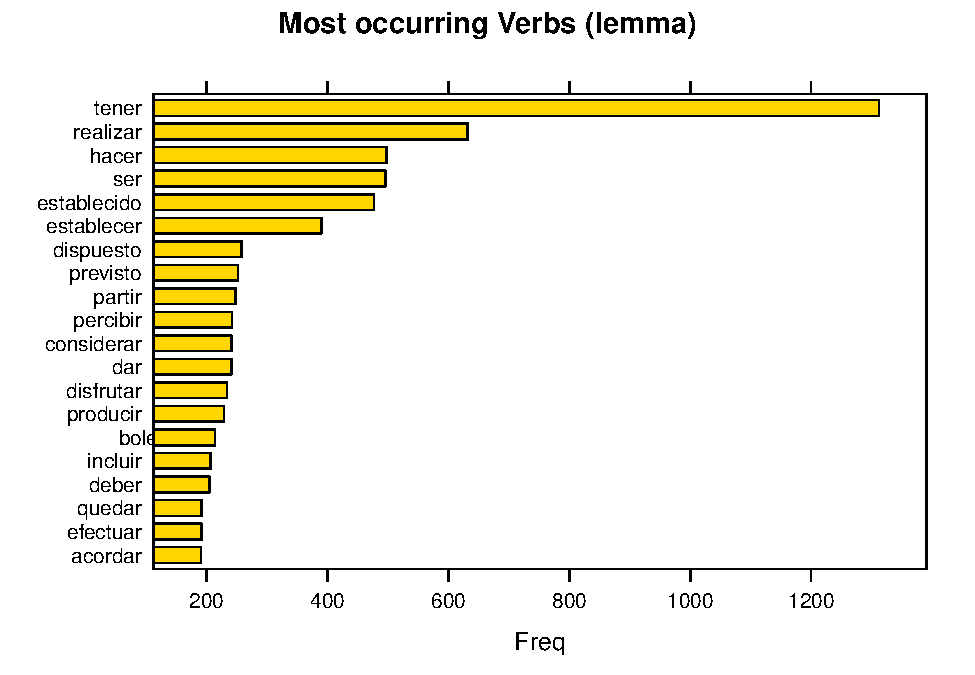
\includegraphics{TFM_files/figure-latex/unnamed-chunk-7-1.pdf}

\begin{Shaded}
\begin{Highlighting}[]
\CommentTok{## Collocation (words following one another)}
\NormalTok{stats <-}\StringTok{ }\KeywordTok{keywords_collocation}\NormalTok{(}\DataTypeTok{x =}\NormalTok{ x, }
                             \DataTypeTok{term =} \StringTok{"token"}\NormalTok{, }\DataTypeTok{group =} \KeywordTok{c}\NormalTok{(}\StringTok{"doc_id"}\NormalTok{, }\StringTok{"paragraph_id"}\NormalTok{, }\StringTok{"sentence_id"}\NormalTok{),}
                             \DataTypeTok{ngram_max =} \DecValTok{4}\NormalTok{)}
\CommentTok{## Co-occurrences: How frequent do words occur in the same sentence, in this case only nouns or adjectives}
\NormalTok{stats <-}\StringTok{ }\KeywordTok{cooccurrence}\NormalTok{(}\DataTypeTok{x =} \KeywordTok{subset}\NormalTok{(x, upos }\OperatorTok\StringTok{ }\KeywordTok{c}\NormalTok{(}\StringTok{"NOUN"}\NormalTok{, }\StringTok{"ADJ"}\NormalTok{)), }
                     \DataTypeTok{term =} \StringTok{"lemma"}\NormalTok{, }\DataTypeTok{group =} \KeywordTok{c}\NormalTok{(}\StringTok{"doc_id"}\NormalTok{, }\StringTok{"paragraph_id"}\NormalTok{, }\StringTok{"sentence_id"}\NormalTok{))}
\CommentTok{## Co-occurrences: How frequent do words follow one another}
\NormalTok{stats <-}\StringTok{ }\KeywordTok{cooccurrence}\NormalTok{(}\DataTypeTok{x =}\NormalTok{ x}\OperatorTok{$}\NormalTok{lemma, }
                     \DataTypeTok{relevant =}\NormalTok{ x}\OperatorTok{$}\NormalTok{upos }\OperatorTok\StringTok{ }\KeywordTok{c}\NormalTok{(}\StringTok{"NOUN"}\NormalTok{, }\StringTok{"ADJ"}\NormalTok{))}
\CommentTok{## Co-occurrences: How frequent do words follow one another even if we would skip 2 words in between}
\NormalTok{stats <-}\StringTok{ }\KeywordTok{cooccurrence}\NormalTok{(}\DataTypeTok{x =}\NormalTok{ x}\OperatorTok{$}\NormalTok{lemma, }
                     \DataTypeTok{relevant =}\NormalTok{ x}\OperatorTok{$}\NormalTok{upos }\OperatorTok\StringTok{ }\KeywordTok{c}\NormalTok{(}\StringTok{"NOUN"}\NormalTok{, }\StringTok{"ADJ"}\NormalTok{), }\DataTypeTok{skipgram =} \DecValTok{2}\NormalTok{)}
\KeywordTok{head}\NormalTok{(stats)}
\end{Highlighting}
\end{Shaded}

\begin{verbatim}
##      term1       term2 cooc
## 1   puesto     trabajo  502
## 2 convenio   colectivo  408
## 3   centro     trabajo  338
## 4    grupo profesional  326
## 5 presente    convenio  257
## 6      día     natural  181
\end{verbatim}

\hypertarget{r-libraryigraph-libraryggraph-libraryggplot2-libraryextrafont-wordnetwork---headstats-30-wordnetwork---graph_from_data_framewordnetwork-ggraphwordnetwork-layout-fr-geom_edge_linkaeswidth-cooc-edge_alpha-cooc-edge_colour-pink-geom_node_textaeslabel-name-col-darkgreen-size-4-theme_graphbase_family-arial-narrow-themelegend.position-none-labstitle-cooccurrences-within-3-words-distance-subtitle-nouns-adjective}{%
\section{\texorpdfstring{\texttt{\{r\}\ \#\ library(igraph)\ \#\ library(ggraph)\ \#\ library(ggplot2)\ \#\ library(extrafont)\ \#\ \ \#\ wordnetwork\ \textless{}-\ head(stats,\ 30)\ \#\ wordnetwork\ \textless{}-\ graph\_from\_data\_frame(wordnetwork)\ \#\ ggraph(wordnetwork,\ layout\ =\ "fr")\ +\ \#\ \ \ geom\_edge\_link(aes(width\ =\ cooc,\ edge\_alpha\ =\ cooc),\ edge\_colour\ =\ "pink")\ +\ \#\ \ \ geom\_node\_text(aes(label\ =\ name),\ col\ =\ "darkgreen",\ size\ =\ 4)\ +\ \#\ \ \ theme\_graph(base\_family\ =\ "Arial\ Narrow")\ +\ \#\ \ \ theme(legend.position\ =\ "none")\ +\ \#\ \ \ labs(title\ =\ "Cooccurrences\ within\ 3\ words\ distance",\ subtitle\ =\ "Nouns\ \&\ Adjective")\ \#}}{\{r\} \# library(igraph) \# library(ggraph) \# library(ggplot2) \# library(extrafont) \#  \# wordnetwork \textless{}- head(stats, 30) \# wordnetwork \textless{}- graph\_from\_data\_frame(wordnetwork) \# ggraph(wordnetwork, layout = "fr") + \#   geom\_edge\_link(aes(width = cooc, edge\_alpha = cooc), edge\_colour = "pink") + \#   geom\_node\_text(aes(label = name), col = "darkgreen", size = 4) + \#   theme\_graph(base\_family = "Arial Narrow") + \#   theme(legend.position = "none") + \#   labs(title = "Cooccurrences within 3 words distance", subtitle = "Nouns \& Adjective") \#}}\label{r-libraryigraph-libraryggraph-libraryggplot2-libraryextrafont-wordnetwork---headstats-30-wordnetwork---graph_from_data_framewordnetwork-ggraphwordnetwork-layout-fr-geom_edge_linkaeswidth-cooc-edge_alpha-cooc-edge_colour-pink-geom_node_textaeslabel-name-col-darkgreen-size-4-theme_graphbase_family-arial-narrow-themelegend.position-none-labstitle-cooccurrences-within-3-words-distance-subtitle-nouns-adjective}}

\begin{Shaded}
\begin{Highlighting}[]
\KeywordTok{library}\NormalTok{(textrank)}
\NormalTok{stats <-}\StringTok{ }\KeywordTok{textrank_keywords}\NormalTok{(x}\OperatorTok{$}\NormalTok{lemma, }
                          \DataTypeTok{relevant =}\NormalTok{ x}\OperatorTok{$}\NormalTok{upos }\OperatorTok\StringTok{ }\KeywordTok{c}\NormalTok{(}\StringTok{"NOUN"}\NormalTok{, }\StringTok{"ADJ"}\NormalTok{), }
                          \DataTypeTok{ngram_max =} \DecValTok{8}\NormalTok{, }\DataTypeTok{sep =} \StringTok{" "}\NormalTok{)}
\NormalTok{stats <-}\StringTok{ }\KeywordTok{subset}\NormalTok{(stats}\OperatorTok{$}\NormalTok{keywords, ngram }\OperatorTok{>}\StringTok{ }\DecValTok{1} \OperatorTok{&}\StringTok{ }\NormalTok{freq }\OperatorTok{>=}\StringTok{ }\DecValTok{5}\NormalTok{)}
\KeywordTok{library}\NormalTok{(wordcloud)}
\end{Highlighting}
\end{Shaded}

\begin{verbatim}
## Loading required package: RColorBrewer
\end{verbatim}

\begin{Shaded}
\begin{Highlighting}[]
\KeywordTok{suppressWarnings}\NormalTok{(}\KeywordTok{wordcloud}\NormalTok{(}\DataTypeTok{words =}\NormalTok{ stats}\OperatorTok{$}\NormalTok{keyword, }\DataTypeTok{freq =}\NormalTok{ stats}\OperatorTok{$}\NormalTok{freq))}
\end{Highlighting}
\end{Shaded}

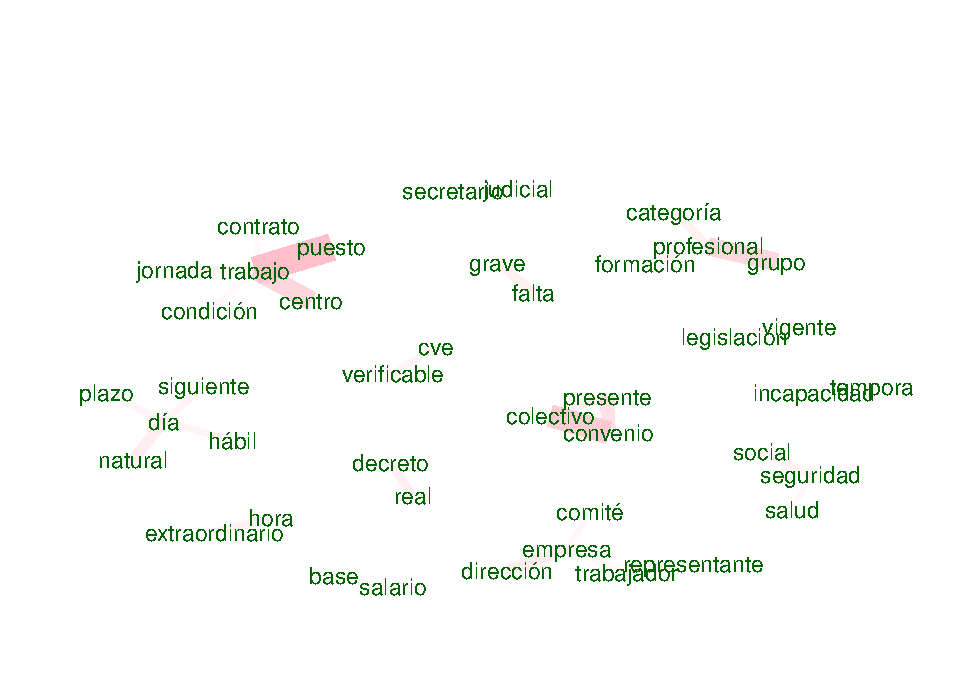
\includegraphics{TFM_files/figure-latex/unnamed-chunk-9-1.pdf}

\begin{Shaded}
\begin{Highlighting}[]
\NormalTok{stats <-}\StringTok{ }\KeywordTok{keywords_rake}\NormalTok{(}\DataTypeTok{x =}\NormalTok{ x, }
                       \DataTypeTok{term =} \StringTok{"lemma"}\NormalTok{, }
                       \DataTypeTok{group =} \StringTok{"doc_id"}\NormalTok{, }
                       \DataTypeTok{relevant =}\NormalTok{ x}\OperatorTok{$}\NormalTok{upos }\OperatorTok\StringTok{ }\KeywordTok{c}\NormalTok{(}\StringTok{"NOUN"}\NormalTok{, }\StringTok{"ADJ"}\NormalTok{))}
\NormalTok{stats}\OperatorTok{$}\NormalTok{key <-}\StringTok{ }\KeywordTok{factor}\NormalTok{(stats}\OperatorTok{$}\NormalTok{keyword, }\DataTypeTok{levels =} \KeywordTok{rev}\NormalTok{(stats}\OperatorTok{$}\NormalTok{keyword))}
\KeywordTok{barchart}\NormalTok{(key }\OperatorTok{~}\StringTok{ }\NormalTok{rake, }
         \DataTypeTok{data =} \KeywordTok{head}\NormalTok{(}\KeywordTok{subset}\NormalTok{(stats, freq }\OperatorTok{>}\StringTok{ }\DecValTok{20}\NormalTok{), }\DecValTok{60}\NormalTok{), }
         \DataTypeTok{col =} \StringTok{"red"}\NormalTok{, }
         \DataTypeTok{main =} \StringTok{"Keywords identified by RAKE"}\NormalTok{, }
         \DataTypeTok{xlab =} \StringTok{"Rake"}\NormalTok{)}
\end{Highlighting}
\end{Shaded}

\includegraphics{TFM_files/figure-latex/unnamed-chunk-10-1.pdf}

Esta figura muestra porcentaje acumulado:

\begin{center}\includegraphics{TFM_files/figure-latex/unnamed-chunk-11-1} \end{center}

Esta figura (mucho más mona) muestra porcentaje acumulado:

\begin{center}\includegraphics{TFM_files/figure-latex/unnamed-chunk-12-1} \end{center}

Tranformacion de UPOS a POS

\begin{Shaded}
\begin{Highlighting}[]
\NormalTok{upos <-}\StringTok{ }\KeywordTok{c}\NormalTok{(}\StringTok{"NOUN"}\NormalTok{,}\StringTok{"ADP"}\NormalTok{,}\StringTok{"DET"}\NormalTok{,}\StringTok{"PUNCT"}\NormalTok{,}\StringTok{"ADJ"}\NormalTok{,}\StringTok{"PROPN"}\NormalTok{,}\StringTok{"VERB"}\NormalTok{,}\StringTok{"NUM"}\NormalTok{,}\StringTok{"CCONJ"}\NormalTok{,}\StringTok{"PRON"}\NormalTok{,}\StringTok{"SCONJ"}\NormalTok{,}\StringTok{"ADV"}\NormalTok{,}\StringTok{"AUX"}\NormalTok{,}\StringTok{"X"}\NormalTok{,}\StringTok{"SYM"}\NormalTok{,}\StringTok{"PART"}\NormalTok{,}\StringTok{"INTJ"}\NormalTok{)}
\KeywordTok{as_phrasemachine}\NormalTok{(upos)}
\end{Highlighting}
\end{Shaded}

\begin{verbatim}
##  [1] "N" "P" "D" "O" "A" "N" "V" "A" "C" "N" "C" "M" "V" "O" "O" "M" "O"
\end{verbatim}

Patron con UPOS

\begin{Shaded}
\begin{Highlighting}[]
\NormalTok{statsUPOS <-}\StringTok{ }\KeywordTok{keywords_phrases}\NormalTok{(}\DataTypeTok{x =}\NormalTok{ x}\OperatorTok{$}\NormalTok{upos, }
                          \DataTypeTok{term =} \KeywordTok{tolower}\NormalTok{(x}\OperatorTok{$}\NormalTok{token), }
                          \CommentTok{#pattern = "(DET|NOUN|ADJ)|(PROPN|NOU|NADJ|AUX)",}
                          \DataTypeTok{pattern =} \StringTok{"((ADJ|NUM)|(NOUN|PROPN|PRON))*(NOUN|PROPN|PRON)(ADP+DET*((ADJ|NUM)|(NOUN|PROPN|PRON))*(NOUN|PROPN|PRON))*"}\NormalTok{, }\CommentTok{#SNP for UPOS}
                          \DataTypeTok{is_regex =} \OtherTok{TRUE}\NormalTok{, }
                          \DataTypeTok{detailed =} \OtherTok{TRUE} \CommentTok{#logical indicating to return the exact positions where the phrase was found (set to TRUE) or just how many times each phrase is occurring (set to FALSE). Defaults to TRUE.}
\NormalTok{                         )}

\CommentTok{#((ADJ|NUM)|(NOUN|PROPN|PRON))*(NOUN|PROPN|PRON)(ADP+DET*((ADJ|NUM)|(NOUN|PROPN|PRON))*(NOUN|PROPN|PRON))*}
\end{Highlighting}
\end{Shaded}

Esta figura muestra porcentaje acumulado:

\begin{center}\includegraphics{TFM_files/figure-latex/unnamed-chunk-15-1} \end{center}

Esta figura (mucho más mona) muestra porcentaje acumulado:

\begin{center}\includegraphics{TFM_files/figure-latex/unnamed-chunk-16-1} \end{center}

\begin{Shaded}
\begin{Highlighting}[]
\KeywordTok{library}\NormalTok{(dplyr)}
\end{Highlighting}
\end{Shaded}

\begin{verbatim}
## 
## Attaching package: 'dplyr'
\end{verbatim}

\begin{verbatim}
## The following objects are masked from 'package:stats':
## 
##     filter, lag
\end{verbatim}

\begin{verbatim}
## The following objects are masked from 'package:base':
## 
##     intersect, setdiff, setequal, union
\end{verbatim}

\begin{Shaded}
\begin{Highlighting}[]
\KeywordTok{library}\NormalTok{(plyr)}
\end{Highlighting}
\end{Shaded}

\begin{verbatim}
## ------------------------------------------------------------------------------
\end{verbatim}

\begin{verbatim}
## You have loaded plyr after dplyr - this is likely to cause problems.
## If you need functions from both plyr and dplyr, please load plyr first, then dplyr:
## library(plyr); library(dplyr)
\end{verbatim}

\begin{verbatim}
## ------------------------------------------------------------------------------
\end{verbatim}

\begin{verbatim}
## 
## Attaching package: 'plyr'
\end{verbatim}

\begin{verbatim}
## The following objects are masked from 'package:dplyr':
## 
##     arrange, count, desc, failwith, id, mutate, rename, summarise,
##     summarize
\end{verbatim}

\begin{Shaded}
\begin{Highlighting}[]
\CommentTok{#Así, podemos obtener la frecuencia de aparicion de un termino específico}
\NormalTok{frequencyOfUPOS <-}\StringTok{ }\KeywordTok{ddply}\NormalTok{(statsUPOS, .(pattern, ngram), nrow)}

\NormalTok{frequencyOfUPOS <-}\StringTok{ }\NormalTok{frequencyOfUPOS[}\KeywordTok{order}\NormalTok{(}\OperatorTok{-}\NormalTok{frequencyOfUPOS}\OperatorTok{$}\NormalTok{V1),]}

\CommentTok{#Así, podemos obtener la frecuencia de aparicion de un termino específico}
\NormalTok{frequencyOfUPOS}
\end{Highlighting}
\end{Shaded}

\begin{verbatim}
##                                       pattern ngram     V1
## 162                                      NOUN     1 110109
## 852                                     PROPN     1  33801
## 785                                      PRON     1  12852
## 255                            NOUNADPDETNOUN     4  11355
## 1008                               PROPNPROPN     2  10878
## 27                                    ADJNOUN     2   5766
## 487                                   NUMNOUN     2   4575
## 1086                          PROPNPROPNPROPN     3   4103
## 1129                     PROPNPROPNPROPNPROPN     4   1837
## 416                                  NOUNPRON     2   1468
## 722                                  NUMPROPN     2   1160
## 421                                 NOUNPROPN     2   1075
## 266                  NOUNADPDETNOUNADPDETNOUN     7   1052
## 313                           NOUNADPDETPROPN     4   1023
## 1148                PROPNPROPNPROPNPROPNPROPN     5    869
## 838                                  PRONPRON     2    853
## 906                          PROPNADPDETPROPN     4    813
## 330                                  NOUNNOUN     2    768
## 795                            PRONADPDETNOUN     4    747
## 242                         NOUNADPDETADJNOUN     5    677
## 885                           PROPNADPDETNOUN     4    647
## 49                          ADJNOUNADPDETNOUN     5    611
## 1037                    PROPNPROPNADPDETPROPN     5    549
## 1159           PROPNPROPNPROPNPROPNPROPNPROPN     6    508
## 753                             NUMPROPNPROPN     3    472
## 134                                   ADJPRON     2    425
## 821                                  PRONNOUN     2    371
## 1163      PROPNPROPNPROPNPROPNPROPNPROPNPROPN     7    324
## 223                               NOUNADJPRON     3    308
## 301                            NOUNADPDETPRON     4    301
## 139                                  ADJPROPN     2    298
## 452                            NOUNPROPNPROPN     3    281
## 185                               NOUNADJNOUN     3    268
## 508                         NUMNOUNADPDETNOUN     5    265
## 323                      NOUNADPDETPROPNPROPN     5    246
## 1165 PROPNPROPNPROPNPROPNPROPNPROPNPROPNPROPN     8    233
## 920                                 PROPNNOUN     2    203
## 228                              NOUNADJPROPN     3    190
## 696                               NUMNUMPROPN     3    167
## 81                                ADJNOUNPRON     3    166
## 584                                NUMNUMNOUN     3    155
## 1030                     PROPNPROPNADPDETNOUN     5    155
## 282                        NOUNADPDETNOUNPRON     5    149
## 273                 NOUNADPDETNOUNADPDETPROPN     7    148
## 1001                                PROPNPRON     2    147
## 463                       NOUNPROPNPROPNPROPN     4    142
## 325           NOUNADPDETPROPNPROPNADPDETPROPN     8    140
## 756                  NUMPROPNPROPNADPDETPROPN     6    137
## 361                               NOUNNUMNOUN     3    134
## 985                             PROPNNUMPROPN     3    127
## 622                             NUMNUMNUMNOUN     4    124
## 944                              PROPNNUMNOUN     3    121
## 765                        NUMPROPNPROPNPROPN     4    119
## 913                     PROPNADPDETPROPNPROPN     5    109
## 685                            NUMNUMNUMPROPN     4    105
## 846                                 PRONPROPN     2    104
## 309                        NOUNADPDETPRONPRON     5    101
## 474                                NUMADJNOUN     3     99
## 643                          NUMNUMNUMNUMNOUN     5     99
## 147                             ADJPROPNPROPN     3     97
## 296                         NOUNADPDETNUMNOUN     5     91
## 274            NOUNADPDETNOUNADPDETPROPNPROPN     8     88
## 678                         NUMNUMNUMNUMPROPN     5     86
## 3                                  ADJADJNOUN     3     81
## 286                       NOUNADPDETNOUNPROPN     5     81
## 798                  PRONADPDETNOUNADPDETNOUN     7     79
## 96                                 ADJNUMNOUN     3     78
## 719                                   NUMPRON     2     77
## 1039               PROPNPROPNADPDETPROPNPROPN     6     77
## 50                ADJNOUNADPDETNOUNADPDETNOUN     8     69
## 848                            PRONPROPNPROPN     3     69
## 708                          NUMNUMPROPNPROPN     4     68
## 991                        PROPNNUMPROPNPROPN     4     67
## 833                              PRONNOUNNOUN     3     66
## 165                            NOUNADJADJNOUN     4     64
## 657                       NUMNUMNUMNUMNUMNOUN     6     59
## 344                        NOUNNOUNADPDETNOUN     5     58
## 689                       NUMNUMNUMPROPNPROPN     5     57
## 789                         PRONADPDETADJNOUN     5     57
## 315                 NOUNADPDETPROPNADPDETNOUN     7     56
## 405                              NOUNNUMPROPN     3     56
## 824                        PRONNOUNADPDETNOUN     5     56
## 244               NOUNADPDETADJNOUNADPDETNOUN     8     54
## 1042                           PROPNPROPNNOUN     3     54
## 151                        ADJPROPNPROPNPROPN     4     52
## 429                      NOUNPROPNADPDETPROPN     5     52
## 779                   NUMPROPNPROPNPROPNPROPN     5     52
## 265               NOUNADPDETNOUNADPDETADJNOUN     8     50
## 235                         NOUNADJPROPNPROPN     4     49
## 275                        NOUNADPDETNOUNNOUN     5     47
## 680                    NUMNUMNUMNUMPROPNPROPN     6     47
## 60                         ADJNOUNADPDETPROPN     5     46
## 468                  NOUNPROPNPROPNPROPNPROPN     5     44
## 569                              NUMNOUNPROPN     3     44
## 673                      NUMNUMNUMNUMNUMPROPN     6     44
## 503                           NUMNOUNADJPROPN     4     42
## 260                     NOUNADPDETNOUNADJPRON     6     40
## 664                    NUMNUMNUMNUMNUMNUMNOUN     7     40
## 526                               NUMNOUNNOUN     3     39
## 450                             NOUNPROPNPRON     3     36
## 902                           PROPNADPDETPRON     4     36
## 52               ADJNOUNADPDETNOUNADPDETPROPN     8     35
## 535                            NUMNOUNNUMNOUN     4     35
## 666                 NUMNUMNUMNUMNUMNUMNUMNOUN     8     35
## 889                 PROPNADPDETNOUNADPDETNOUN     7     35
## 670                   NUMNUMNUMNUMNUMNUMPROPN     7     34
## 47                       ADJNOUNADPDETADJNOUN     6     33
## 510               NUMNOUNADPDETNOUNADPDETNOUN     8     33
## 303                  NOUNADPDETPRONADPDETNOUN     7     32
## 782              NUMPROPNPROPNPROPNPROPNPROPN     6     32
## 193                     NOUNADJNOUNADPDETNOUN     6     31
## 238                    NOUNADJPROPNPROPNPROPN     5     31
## 1075                       PROPNPROPNNUMPROPN     4     31
## 712                     NUMNUMPROPNPROPNPROPN     5     30
## 1082                           PROPNPROPNPRON     3     30
## 64                                ADJNOUNNOUN     3     29
## 583                             NUMNUMADJNOUN     4     29
## 621                          NUMNUMNUMADJNOUN     5     29
## 642                       NUMNUMNUMNUMADJNOUN     6     28
## 844                              PRONPRONPRON     3     28
## 690                  NUMNUMNUMPROPNPROPNPROPN     6     27
## 424                       NOUNPROPNADPDETNOUN     5     26
## 1102               PROPNPROPNPROPNADPDETPROPN     6     26
## 271                  NOUNADPDETNOUNADPDETPRON     7     25
## 668                NUMNUMNUMNUMNUMNUMNUMPROPN     8     25
## 1055                        PROPNPROPNNUMNOUN     4     25
## 859                              PROPNADJNOUN     3     24
## 916          PROPNADPDETPROPNPROPNADPDETPROPN     8     24
## 993                   PROPNNUMPROPNPROPNPROPN     5     24
## 18                                ADJADJPROPN     3     23
## 83                               ADJNOUNPROPN     3     23
## 674                 NUMNUMNUMNUMNUMPROPNPROPN     7     23
## 681               NUMNUMNUMNUMPROPNPROPNPROPN     7     23
## 917                PROPNADPDETPROPNPROPNPROPN     6     23
## 258                     NOUNADPDETNOUNADJNOUN     6     22
## 394                     NOUNNUMNUMNUMNUMPROPN     6     22
## 63                    ADJNOUNADPDETPROPNPROPN     6     21
## 420                              NOUNPRONPRON     3     21
## 418                              NOUNPRONNOUN     3     20
## 816                           PRONADPDETPROPN     4     20
## 1040          PROPNPROPNADPDETPROPNPROPNPROPN     7     20
## 19                           ADJADJPROPNPROPN     4     19
## 35                             ADJNOUNADJNOUN     4     19
## 156                   ADJPROPNPROPNPROPNPROPN     5     19
## 292                  NOUNADPDETNOUNPROPNPROPN     6     19
## 295                      NOUNADPDETNUMADJNOUN     6     19
## 403                               NOUNNUMPRON     3     19
## 409                         NOUNNUMPROPNPROPN     4     19
## 567                               NUMNOUNPRON     3     19
## 881                        PROPNADPDETADJNOUN     5     19
## 387                      NOUNNUMNUMNUMNUMNOUN     6     18
## 506                      NUMNOUNADPDETADJNOUN     6     18
## 715                NUMNUMPROPNPROPNPROPNPROPN     6     18
## 1105                      PROPNPROPNPROPNNOUN     4     18
## 17                                 ADJADJPRON     3     17
## 318                NOUNADPDETPROPNADPDETPROPN     7     17
## 671              NUMNUMNUMNUMNUMNUMPROPNPROPN     8     17
## 692             NUMNUMNUMPROPNPROPNPROPNPROPN     7     17
## 783         NUMPROPNPROPNPROPNPROPNPROPNPROPN     7     17
## 938                            PROPNNOUNPROPN     3     17
## 1122                  PROPNPROPNPROPNNUMPROPN     5     17
## 178                           NOUNADJADJPROPN     4     16
## 504                      NUMNOUNADJPROPNPROPN     5     16
## 516                      NUMNOUNADPDETNUMNOUN     6     16
## 1076                  PROPNPROPNNUMPROPNPROPN     5     16
## 58                          ADJNOUNADPDETPRON     5     15
## 177                            NOUNADJADJPRON     4     15
## 205                            NOUNADJNUMNOUN     4     15
## 327                 NOUNADPDETPROPNPROPNPROPN     6     15
## 370                        NOUNNUMNOUNNUMNOUN     5     15
## 410                    NOUNNUMPROPNPROPNPROPN     5     15
## 471             NOUNPROPNPROPNPROPNPROPNPROPN     6     15
## 537                     NUMNOUNNUMNOUNNUMNOUN     6     15
## 1014                        PROPNPROPNADJNOUN     4     15
## 357                             NOUNNOUNPROPN     3     14
## 396                NOUNNUMNUMNUMNUMPROPNPROPN     7     14
## 682          NUMNUMNUMNUMPROPNPROPNPROPNPROPN     8     14
## 809                         PRONADPDETNUMNOUN     5     14
## 505                 NUMNOUNADJPROPNPROPNPROPN     6     13
## 726                           NUMPROPNNUMNOUN     4     13
## 812                            PRONADPDETPRON     4     13
## 939                       PROPNNOUNPROPNPROPN     4     13
## 1101                PROPNPROPNPROPNADPDETNOUN     6     13
## 137                               ADJPRONNOUN     3     12
## 179                      NOUNADJADJPROPNPROPN     5     12
## 350                              NOUNNOUNNOUN     3     12
## 363                       NOUNNUMNOUNADJPROPN     5     12
## 492                            NUMNOUNADJNOUN     4     12
## 579                         NUMNOUNPROPNPROPN     4     12
## 745                          NUMPROPNNUMPROPN     4     12
## 802                 PRONADPDETNOUNADPDETPROPN     7     12
## 834                              PRONNOUNPRON     3     12
## 875                             PROPNADJPROPN     3     12
## 908                PROPNADPDETPROPNADPDETNOUN     7     12
## 940                  PROPNNOUNPROPNPROPNPROPN     5     12
## 21                      ADJADJPROPNPROPNPROPN     5     11
## 142                       ADJPROPNADPDETPROPN     5     11
## 249                      NOUNADPDETADJNUMNOUN     6     11
## 261                    NOUNADPDETNOUNADJPROPN     6     11
## 269             NOUNADPDETNOUNADPDETNOUNPROPN     8     11
## 417                        NOUNPRONADPDETNOUN     5     11
## 560                           NUMNOUNNUMPROPN     4     11
## 675            NUMNUMNUMNUMNUMPROPNPROPNPROPN     8     11
## 826              PRONNOUNADPDETNOUNADPDETNOUN     8     11
## 904                       PROPNADPDETPRONPRON     5     11
## 970                     PROPNNUMNUMNUMNUMNOUN     6     11
## 1091                   PROPNPROPNPROPNADJNOUN     5     11
## 1123             PROPNPROPNPROPNNUMPROPNPROPN     6     11
## 335                           NOUNNOUNADJNOUN     4     10
## 348                       NOUNNOUNADPDETPROPN     5     10
## 383                         NOUNNUMNUMNUMNOUN     5     10
## 518                         NUMNOUNADPDETPRON     5     10
## 580                    NUMNOUNPROPNPROPNPROPN     5     10
## 717           NUMNUMPROPNPROPNPROPNPROPNPROPN     7     10
## 784    NUMPROPNPROPNPROPNPROPNPROPNPROPNPROPN     8     10
## 900                        PROPNADPDETNUMNOUN     5     10
## 1078             PROPNPROPNNUMPROPNPROPNPROPN     6     10
## 1111                   PROPNPROPNPROPNNUMNOUN     5     10
## 1144             PROPNPROPNPROPNPROPNNUMPROPN     6     10
## 123                               ADJNUMPROPN     3      9
## 231                   NOUNADJPROPNADPDETPROPN     6      9
## 248                     NOUNADPDETADJNOUNPRON     6      9
## 345              NOUNNOUNADPDETNOUNADPDETNOUN     8      9
## 371                 NOUNNUMNOUNNUMNOUNNUMNOUN     7      9
## 389                   NOUNNUMNUMNUMNUMNUMNOUN     7      9
## 538              NUMNOUNNUMNOUNNUMNOUNNUMNOUN     8      9
## 693        NUMNUMNUMPROPNPROPNPROPNPROPNPROPN     8      9
## 788                               PRONADJNOUN     3      9
## 805                        PRONADPDETNOUNPRON     5      9
## 928                       PROPNNOUNADPDETNOUN     5      9
## 1052                      PROPNPROPNNOUNPROPN     4      9
## 42                             ADJNOUNADJPRON     4      8
## 112                       ADJNUMNUMNUMNUMNOUN     6      8
## 241               NOUNADJPROPNPROPNPROPNPROPN     6      8
## 256                  NOUNADPDETNOUNADJADJNOUN     7      8
## 272              NOUNADPDETNOUNADPDETPRONPRON     8      8
## 386                   NOUNNUMNUMNUMNUMADJNOUN     7      8
## 563                      NUMNOUNNUMPROPNPROPN     5      8
## 581               NUMNOUNPROPNPROPNPROPNPROPN     6      8
## 749                     NUMPROPNNUMPROPNPROPN     5      8
## 918           PROPNADPDETPROPNPROPNPROPNPROPN     7      8
## 929                      PROPNNOUNADPDETPROPN     5      8
## 930                 PROPNNOUNADPDETPROPNPROPN     6      8
## 998              PROPNNUMPROPNPROPNPROPNPROPN     6      8
## 1004                            PROPNPRONPRON     3      8
## 1041     PROPNPROPNADPDETPROPNPROPNPROPNPROPN     8      8
## 1053                 PROPNPROPNNOUNPROPNPROPN     5      8
## 1054            PROPNPROPNNOUNPROPNPROPNPROPN     6      8
## 1138          PROPNPROPNPROPNPROPNADPDETPROPN     7      8
## 1140                 PROPNPROPNPROPNPROPNNOUN     5      8
## 11                       ADJADJNOUNADPDETNOUN     6      7
## 24                 ADJADJPROPNPROPNPROPNPROPN     6      7
## 43                            ADJNOUNADJPROPN     4      7
## 75                    ADJNOUNNUMNUMNUMNUMNOUN     7      7
## 77                   ADJNOUNNUMNUMNUMNUMPROPN     7      7
## 425             NOUNPROPNADPDETNOUNADPDETNOUN     8      7
## 478                NUMADJNOUNNUMNUMNUMNUMNOUN     8      7
## 551                   NUMNOUNNUMNUMNUMNUMNOUN     7      7
## 564                 NUMNOUNNUMPROPNPROPNPROPN     6      7
## 606                NUMNUMNOUNNUMNUMNUMNUMNOUN     8      7
## 614                           NUMNUMNOUNPROPN     4      7
## 656                    NUMNUMNUMNUMNUMADJNOUN     7      7
## 718      NUMNUMPROPNPROPNPROPNPROPNPROPNPROPN     8      7
## 819                      PRONADPDETPROPNPROPN     5      7
## 840                        PRONPRONADPDETNOUN     5      7
## 854                          PROPNADJADJPROPN     4      7
## 855                     PROPNADJADJPROPNPROPN     5      7
## 871                           PROPNADJNUMNOUN     4      7
## 949                    PROPNNUMNOUNADPDETNOUN     6      7
## 968                        PROPNNUMNUMNUMNOUN     5      7
## 969                  PROPNNUMNUMNUMNUMADJNOUN     7      7
## 977                       PROPNNUMNUMNUMPROPN     5      7
## 1010                    PROPNPROPNADJADJPROPN     5      7
## 1011               PROPNPROPNADJADJPROPNPROPN     6      7
## 1103          PROPNPROPNPROPNADPDETPROPNPROPN     7      7
## 78              ADJNOUNNUMNUMNUMNUMPROPNPROPN     8      6
## 90                          ADJNOUNPROPNPROPN     4      6
## 130                          ADJNUMPROPNPROPN     4      6
## 136                         ADJPRONADPDETNOUN     5      6
## 138                               ADJPRONPRON     3      6
## 191                       NOUNADJNOUNADJPROPN     5      6
## 202                          NOUNADJNOUNPROPN     4      6
## 220                           NOUNADJNUMPROPN     4      6
## 227                           NOUNADJPRONPRON     4      6
## 246              NOUNADPDETADJNOUNADPDETPROPN     8      6
## 277              NOUNADPDETNOUNNOUNADPDETNOUN     8      6
## 279                     NOUNADPDETNOUNNUMNOUN     6      6
## 290                   NOUNADPDETNOUNPROPNPRON     6      6
## 293             NOUNADPDETNOUNPROPNPROPNPROPN     7      6
## 343                     NOUNNOUNADPDETADJNOUN     6      6
## 349                  NOUNNOUNADPDETPROPNPROPN     6      6
## 365                           NOUNNUMNOUNNOUN     4      6
## 377                          NOUNNUMNOUNPROPN     4      6
## 392                  NOUNNUMNUMNUMNUMNUMPROPN     7      6
## 397           NOUNNUMNUMNUMNUMPROPNPROPNPROPN     8      6
## 413               NOUNNUMPROPNPROPNPROPNPROPN     6      6
## 433                             NOUNPROPNNOUN     3      6
## 472        NOUNPROPNPROPNPROPNPROPNPROPNPROPN     7      6
## 479               NUMADJNOUNNUMNUMNUMNUMPROPN     8      6
## 548                      NUMNOUNNUMNUMNUMNOUN     6      6
## 663                 NUMNUMNUMNUMNUMNUMADJNOUN     8      6
## 738               NUMPROPNNUMNUMNUMNUMADJNOUN     8      6
## 856                PROPNADJADJPROPNPROPNPROPN     6      6
## 961                         PROPNNUMNOUNPROPN     4      6
## 974                    PROPNNUMNUMNUMNUMPROPN     6      6
## 981                          PROPNNUMNUMPROPN     4      6
## 1012          PROPNPROPNADJADJPROPNPROPNPROPN     7      6
## 1088               PROPNPROPNPROPNADJADJPROPN     6      6
## 1089          PROPNPROPNPROPNADJADJPROPNPROPN     7      6
## 1090     PROPNPROPNPROPNADJADJPROPNPROPNPROPN     8      6
## 1124        PROPNPROPNPROPNNUMPROPNPROPNPROPN     7      6
## 1126                      PROPNPROPNPROPNPRON     4      6
## 1131          PROPNPROPNPROPNPROPNADJADJPROPN     7      6
## 1132     PROPNPROPNPROPNPROPNADJADJPROPNPROPN     8      6
## 1139     PROPNPROPNPROPNPROPNADPDETPROPNPROPN     8      6
## 1145        PROPNPROPNPROPNPROPNNUMPROPNPROPN     7      6
## 1150     PROPNPROPNPROPNPROPNPROPNADJADJPROPN     8      6
## 30                         ADJNOUNADJADJPROPN     5      5
## 31                    ADJNOUNADJADJPROPNPROPN     6      5
## 51                ADJNOUNADPDETNOUNADPDETPRON     8      5
## 59                      ADJNOUNADPDETPRONPRON     6      5
## 68                      ADJNOUNNOUNADPDETNOUN     6      5
## 159              ADJPROPNPROPNPROPNPROPNPROPN     6      5
## 160         ADJPROPNPROPNPROPNPROPNPROPNPROPN     7      5
## 181                 NOUNADJADJPROPNPROPNPROPN     6      5
## 222                      NOUNADJNUMPROPNPROPN     5      5
## 267              NOUNADPDETNOUNADPDETNOUNNOUN     8      5
## 268              NOUNADPDETNOUNADPDETNOUNPRON     8      5
## 288            NOUNADPDETNOUNPROPNADPDETPROPN     8      5
## 320                       NOUNADPDETPROPNPRON     5      5
## 364                     NOUNNUMNOUNADPDETNOUN     6      5
## 393             NOUNNUMNUMNUMNUMNUMPROPNPROPN     8      5
## 414          NOUNNUMPROPNPROPNPROPNPROPNPROPN     7      5
## 432                 NOUNPROPNADPDETPROPNPROPN     6      5
## 473   NOUNPROPNPROPNPROPNPROPNPROPNPROPNPROPN     8      5
## 475                      NUMADJNOUNADPDETNOUN     6      5
## 496                         NUMNOUNADJNUMNOUN     5      5
## 523                        NUMNOUNADPDETPROPN     5      5
## 552                NUMNOUNNUMNUMNUMNUMNUMNOUN     8      5
## 554                  NUMNOUNNUMNUMNUMNUMPROPN     7      5
## 555             NUMNOUNNUMNUMNUMNUMPROPNPROPN     8      5
## 605                   NUMNUMNOUNNUMNUMNUMNOUN     7      5
## 607               NUMNUMNOUNNUMNUMNUMNUMPROPN     8      5
## 634                NUMNUMNUMNOUNNUMNUMNUMNOUN     8      5
## 836                               PRONNUMNOUN     3      5
## 845                             PRONPRONPROPN     3      5
## 894                PROPNADPDETNOUNADPDETPROPN     7      5
## 898                      PROPNADPDETNOUNPROPN     5      5
## 905                  PROPNADPDETPRONPRONPROPN     6      5
## 931                             PROPNNOUNNOUN     3      5
## 978                  PROPNNUMNUMNUMPROPNPROPN     6      5
## 984                              PROPNNUMPRON     3      5
## 1133              PROPNPROPNPROPNPROPNADJNOUN     6      5
## 1137           PROPNPROPNPROPNPROPNADPDETNOUN     7      5
## 1151         PROPNPROPNPROPNPROPNPROPNADJNOUN     7      5
## 1153     PROPNPROPNPROPNPROPNPROPNADPDETPROPN     8      5
## 1160    PROPNPROPNPROPNPROPNPROPNPROPNADJNOUN     8      5
## 25            ADJADJPROPNPROPNPROPNPROPNPROPN     7      4
## 26       ADJADJPROPNPROPNPROPNPROPNPROPNPROPN     8      4
## 33               ADJNOUNADJADJPROPNPROPNPROPN     7      4
## 34          ADJNOUNADJADJPROPNPROPNPROPNPROPN     8      4
## 37                   ADJNOUNADJNOUNADPDETNOUN     7      4
## 55                      ADJNOUNADPDETNOUNPRON     6      4
## 114                   ADJNUMNUMNUMNUMNUMPROPN     7      4
## 119                         ADJNUMNUMNUMPROPN     5      4
## 161    ADJPROPNPROPNPROPNPROPNPROPNPROPNPROPN     8      4
## 183            NOUNADJADJPROPNPROPNPROPNPROPN     7      4
## 184       NOUNADJADJPROPNPROPNPROPNPROPNPROPN     8      4
## 188                        NOUNADJNOUNADJNOUN     5      4
## 201                           NOUNADJNOUNPRON     4      4
## 225                     NOUNADJPRONADPDETNOUN     6      4
## 263               NOUNADPDETNOUNADJPROPNPROPN     7      4
## 270               NOUNADPDETNOUNADPDETNUMNOUN     8      4
## 298               NOUNADPDETNUMNOUNADPDETNOUN     8      4
## 310                    NOUNADPDETPRONPRONPRON     6      4
## 419                    NOUNPRONNOUNADPDETNOUN     6      4
## 430            NOUNPROPNADPDETPROPNADPDETNOUN     8      4
## 462                        NOUNPROPNPROPNPRON     4      4
## 519               NUMNOUNADPDETPRONADPDETNOUN     8      4
## 582          NUMNOUNPROPNPROPNPROPNPROPNPROPN     7      4
## 592                        NUMNUMNOUNADJPROPN     5      4
## 598                         NUMNUMNOUNNUMNOUN     5      4
## 617                      NUMNUMNOUNPROPNPROPN     5      4
## 618                 NUMNUMNOUNPROPNPROPNPROPN     6      4
## 619            NUMNUMNOUNPROPNPROPNPROPNPROPN     7      4
## 620       NUMNUMNOUNPROPNPROPNPROPNPROPNPROPN     8      4
## 628                      NUMNUMNUMNOUNNUMNOUN     6      4
## 636                        NUMNUMNUMNOUNPROPN     5      4
## 651                     NUMNUMNUMNUMNOUNPROPN     6      4
## 660                  NUMNUMNUMNUMNUMNOUNPROPN     7      4
## 665               NUMNUMNUMNUMNUMNUMNOUNPROPN     8      4
## 723                        NUMPROPNADPDETNOUN     5      4
## 750                NUMPROPNNUMPROPNPROPNPROPN     6      4
## 751           NUMPROPNNUMPROPNPROPNPROPNPROPN     7      4
## 759             NUMPROPNPROPNNUMNUMNUMNUMNOUN     8      4
## 773                 NUMPROPNPROPNPROPNNUMNOUN     6      4
## 791               PRONADPDETADJNOUNADPDETNOUN     8      4
## 806                       PRONADPDETNOUNPROPN     5      4
## 828                   PRONNOUNADPDETNOUNPROPN     6      4
## 860                   PROPNADJNOUNADJADJPROPN     6      4
## 861              PROPNADJNOUNADJADJPROPNPROPN     7      4
## 862         PROPNADJNOUNADJADJPROPNPROPNPROPN     8      4
## 876                        PROPNADJPROPNPROPN     4      4
## 897                       PROPNADPDETNOUNPRON     5      4
## 924                         PROPNNOUNADJPROPN     4      4
## 951                          PROPNNUMNOUNNOUN     4      4
## 955                       PROPNNUMNOUNNUMNOUN     5      4
## 971                  PROPNNUMNUMNUMNUMNUMNOUN     7      4
## 975               PROPNNUMNUMNUMNUMPROPNPROPN     7      4
## 1005                           PROPNPRONPROPN     3      4
## 1015             PROPNPROPNADJNOUNADJADJPROPN     7      4
## 1016        PROPNPROPNADJNOUNADJADJPROPNPROPN     8      4
## 1023                       PROPNPROPNADJPROPN     4      4
## 1034                PROPNPROPNADPDETNOUNPROPN     6      4
## 1035                  PROPNPROPNADPDETNUMNOUN     6      4
## 1046                       PROPNPROPNNOUNNOUN     4      4
## 1068               PROPNPROPNNUMNUMNUMNUMNOUN     7      4
## 1072                    PROPNPROPNNUMNUMPROPN     5      4
## 1083                      PROPNPROPNPRONPROPN     4      4
## 1092        PROPNPROPNPROPNADJNOUNADJADJPROPN     8      4
## 1097                  PROPNPROPNPROPNADJPROPN     5      4
## 22               ADJADJPROPNPROPNPROPNADJNOUN     7      3
## 28                          ADJNOUNADJADJNOUN     5      3
## 61               ADJNOUNADPDETPROPNADPDETNOUN     8      3
## 74                 ADJNOUNNUMNUMNUMNUMADJNOUN     8      3
## 91                     ADJNOUNPROPNPROPNPROPN     5      3
## 101                      ADJNUMNOUNADPDETNOUN     6      3
## 102                           ADJNUMNOUNPROPN     4      3
## 113                    ADJNUMNUMNUMNUMNUMNOUN     7      3
## 140                        ADJPROPNADPDETNOUN     5      3
## 152                 ADJPROPNPROPNPROPNADJNOUN     6      3
## 171                  NOUNADJADJNOUNADPDETNOUN     7      3
## 194                    NOUNADJNOUNADPDETPROPN     6      3
## 217                NOUNADJNUMNUMNUMNUMNUMNOUN     8      3
## 245               NOUNADPDETADJNOUNADPDETPRON     8      3
## 247                     NOUNADPDETADJNOUNNOUN     6      3
## 250                         NOUNADPDETADJPRON     5      3
## 251                        NOUNADPDETADJPROPN     5      3
## 264          NOUNADPDETNOUNADJPROPNPROPNPROPN     8      3
## 287             NOUNADPDETNOUNPROPNADPDETNOUN     8      3
## 329            NOUNADPDETPROPNPROPNPROPNPROPN     7      3
## 353                           NOUNNOUNNUMNOUN     4      3
## 360                            NOUNNUMADJNOUN     4      3
## 390                NOUNNUMNUMNUMNUMNUMNUMNOUN     8      3
## 391               NOUNNUMNUMNUMNUMNUMNUMPROPN     8      3
## 398                        NOUNNUMNUMNUMPROPN     5      3
## 406                       NOUNNUMPROPNNUMNOUN     5      3
## 415     NOUNNUMPROPNPROPNPROPNPROPNPROPNPROPN     8      3
## 451                         NOUNPROPNPRONPRON     4      3
## 453                 NOUNPROPNPROPNADPDETPROPN     6      3
## 455                        NOUNPROPNPROPNNOUN     4      3
## 502                            NUMNOUNADJPRON     4      3
## 533                          NUMNOUNNOUNPROPN     4      3
## 536                    NUMNOUNNUMNOUNADJPROPN     6      3
## 553               NUMNOUNNUMNUMNUMNUMNUMPROPN     8      3
## 570                          NUMNOUNPROPNNOUN     4      3
## 593                   NUMNUMNOUNADJPROPNPROPN     6      3
## 599                  NUMNUMNOUNNUMNOUNNUMNOUN     7      3
## 629               NUMNUMNUMNOUNNUMNOUNNUMNOUN     8      3
## 639                   NUMNUMNUMNOUNPROPNPROPN     6      3
## 640              NUMNUMNUMNOUNPROPNPROPNPROPN     7      3
## 641         NUMNUMNUMNOUNPROPNPROPNPROPNPROPN     8      3
## 649                   NUMNUMNUMNUMNOUNNUMNOUN     7      3
## 654                NUMNUMNUMNUMNOUNPROPNPROPN     7      3
## 655           NUMNUMNUMNUMNOUNPROPNPROPNPROPN     8      3
## 659                NUMNUMNUMNUMNUMNOUNNUMNOUN     8      3
## 662             NUMNUMNUMNUMNUMNOUNPROPNPROPN     8      3
## 780           NUMPROPNPROPNPROPNPROPNNUMPROPN     7      3
## 801                  PRONADPDETNOUNADPDETPRON     7      3
## 814                        PRONADPDETPRONPRON     5      3
## 817                 PRONADPDETPROPNADPDETNOUN     7      3
## 843                              PRONPRONNOUN     3      3
## 847                      PRONPROPNADPDETPROPN     5      3
## 857         PROPNADJADJPROPNPROPNPROPNADJNOUN     8      3
## 858           PROPNADJADJPROPNPROPNPROPNPROPN     7      3
## 886                    PROPNADPDETNOUNADJNOUN     6      3
## 910               PROPNADPDETPROPNADPDETPROPN     7      3
## 919      PROPNADPDETPROPNPROPNPROPNPROPNPROPN     8      3
## 925                    PROPNNOUNADJPROPNPROPN     5      3
## 932                         PROPNNOUNNOUNNOUN     4      3
## 936                          PROPNNOUNNUMNOUN     4      3
## 948                      PROPNNUMNOUNADJPROPN     5      3
## 956                PROPNNUMNOUNNUMNOUNNUMNOUN     7      3
## 976          PROPNNUMNUMNUMNUMPROPNPROPNPROPN     8      3
## 999         PROPNNUMPROPNPROPNPROPNPROPNPROPN     7      3
## 1006                PROPNPRONPROPNADPDETPROPN     6      3
## 1013     PROPNPROPNADJADJPROPNPROPNPROPNPROPN     8      3
## 1047                   PROPNPROPNNOUNNOUNNOUN     5      3
## 1061                   PROPNPROPNNUMNOUNPROPN     5      3
## 1070                 PROPNPROPNNUMNUMNUMPROPN     6      3
## 1080        PROPNPROPNNUMPROPNPROPNPROPNPROPN     7      3
## 1084           PROPNPROPNPRONPROPNADPDETPROPN     7      3
## 1104     PROPNPROPNPROPNADPDETPROPNPROPNPROPN     8      3
## 1141              PROPNPROPNPROPNPROPNNUMNOUN     6      3
## 1147                 PROPNPROPNPROPNPROPNPRON     5      3
## 1152      PROPNPROPNPROPNPROPNPROPNADPDETNOUN     8      3
## 1                               ADJADJADJNOUN     4      2
## 5                           ADJADJNOUNADJNOUN     5      2
## 39                        ADJNOUNADJNOUNPROPN     5      2
## 48                   ADJNOUNADPDETADJNOUNPRON     7      2
## 56                     ADJNOUNADPDETNOUNPROPN     6      2
## 57                       ADJNOUNADPDETNUMNOUN     6      2
## 73                             ADJNOUNNUMNOUN     4      2
## 84                    ADJNOUNPROPNADPDETPROPN     6      2
## 92                ADJNOUNPROPNPROPNPROPNPROPN     6      2
## 97                       ADJNUMNOUNADJNUMNOUN     6      2
## 98                         ADJNUMNOUNADJPROPN     5      2
## 106                             ADJNUMNUMNOUN     4      2
## 116                      ADJNUMNUMNUMNUMPROPN     6      2
## 143                  ADJPROPNADPDETPROPNPROPN     6      2
## 144                              ADJPROPNNOUN     3      2
## 146                              ADJPROPNPRON     3      2
## 163                         NOUNADJADJADJNOUN     5      2
## 167                     NOUNADJADJNOUNADJNOUN     6      2
## 196                           NOUNADJNOUNNOUN     4      2
## 206                  NOUNADJNUMNOUNADJNUMNOUN     7      2
## 211                         NOUNADJNUMNUMNOUN     5      2
## 218               NOUNADJNUMNUMNUMNUMNUMPROPN     8      2
## 226                           NOUNADJPRONNOUN     4      2
## 229                    NOUNADJPROPNADPDETNOUN     6      2
## 232                          NOUNADJPROPNNOUN     4      2
## 283              NOUNADPDETNOUNPRONADPDETNOUN     8      2
## 285                    NOUNADPDETNOUNPRONPRON     6      2
## 294        NOUNADPDETNOUNPROPNPROPNPROPNPROPN     8      2
## 299                     NOUNADPDETNUMNOUNPRON     6      2
## 306                 NOUNADPDETPRONADPDETPROPN     7      2
## 307            NOUNADPDETPRONADPDETPROPNPROPN     8      2
## 308                        NOUNADPDETPRONNOUN     5      2
## 314              NOUNADPDETPROPNADPDETADJNOUN     8      2
## 319           NOUNADPDETPROPNADPDETPROPNPROPN     8      2
## 324            NOUNADPDETPROPNPROPNADPDETNOUN     8      2
## 331                        NOUNNOUNADJADJNOUN     5      2
## 339                           NOUNNOUNADJPRON     4      2
## 340                          NOUNNOUNADJPROPN     4      2
## 356                              NOUNNOUNPRON     3      2
## 372                NOUNNUMNOUNNUMNOUNNUMPROPN     7      2
## 373           NOUNNUMNOUNNUMNOUNNUMPROPNPROPN     8      2
## 374                       NOUNNUMNOUNNUMPROPN     5      2
## 375                  NOUNNUMNOUNNUMPROPNPROPN     6      2
## 376             NOUNNUMNOUNNUMPROPNPROPNPROPN     7      2
## 380                            NOUNNUMNUMNOUN     4      2
## 401                           NOUNNUMNUMPROPN     4      2
## 407               NOUNNUMPROPNNUMNOUNNUMPROPN     7      2
## 423                    NOUNPROPNADPDETADJNOUN     6      2
## 434                   NOUNPROPNNOUNADPDETNOUN     6      2
## 446                         NOUNPROPNNUMPROPN     4      2
## 447                    NOUNPROPNNUMPROPNPROPN     5      2
## 448               NOUNPROPNNUMPROPNPROPNPROPN     6      2
## 449       NOUNPROPNNUMPROPNPROPNPROPNNUMPROPN     8      2
## 454            NOUNPROPNPROPNADPDETPROPNPROPN     7      2
## 457                    NOUNPROPNPROPNNOUNNOUN     5      2
## 458                NOUNPROPNPROPNNOUNNOUNNOUN     6      2
## 470       NOUNPROPNPROPNPROPNPROPNNUMNUMPROPN     8      2
## 481                             NUMADJNUMNOUN     4      2
## 493                    NUMNOUNADJNOUNADJPROPN     6      2
## 497               NUMNOUNADJNUMNOUNADJNUMNOUN     8      2
## 511              NUMNOUNADPDETNOUNADPDETPROPN     8      2
## 513                     NUMNOUNADPDETNOUNPRON     6      2
## 524                   NUMNOUNADPDETPROPNPROPN     6      2
## 530                     NUMNOUNNOUNADPDETNOUN     6      2
## 539             NUMNOUNNUMNOUNNUMNOUNNUMPROPN     8      2
## 540                    NUMNOUNNUMNOUNNUMPROPN     6      2
## 541               NUMNOUNNUMNOUNNUMPROPNPROPN     7      2
## 542          NUMNOUNNUMNOUNNUMPROPNPROPNPROPN     8      2
## 550                NUMNOUNNUMNUMNUMNUMADJNOUN     8      2
## 556                     NUMNOUNNUMNUMNUMPROPN     6      2
## 568                           NUMNOUNPRONPRON     4      2
## 576                      NUMNOUNPROPNNUMPROPN     5      2
## 577                 NUMNOUNPROPNNUMPROPNPROPN     6      2
## 578            NUMNOUNPROPNNUMPROPNPROPNPROPN     7      2
## 589                      NUMNUMNOUNADJNUMNOUN     6      2
## 594              NUMNUMNOUNADJPROPNPROPNPROPN     7      2
## 595                      NUMNUMNOUNADPDETNOUN     6      2
## 597                            NUMNUMNOUNNOUN     4      2
## 608                  NUMNUMNOUNNUMNUMNUMPROPN     7      2
## 624                   NUMNUMNUMNOUNADJNUMNOUN     7      2
## 625                     NUMNUMNUMNOUNADJPROPN     6      2
## 635               NUMNUMNUMNOUNNUMNUMNUMPROPN     8      2
## 645                NUMNUMNUMNUMNOUNADJNUMNOUN     8      2
## 646                  NUMNUMNUMNUMNOUNADJPROPN     7      2
## 658               NUMNUMNUMNUMNUMNOUNADJPROPN     8      2
## 686                     NUMNUMNUMPROPNNUMNOUN     6      2
## 688              NUMNUMNUMPROPNNUMNUMNUMPROPN     8      2
## 691           NUMNUMNUMPROPNPROPNPROPNNUMNOUN     8      2
## 694                                NUMNUMPRON     3      2
## 700                        NUMNUMPROPNNUMNOUN     5      2
## 702               NUMNUMPROPNNUMNUMNUMNUMNOUN     8      2
## 704                 NUMNUMPROPNNUMNUMNUMPROPN     7      2
## 706                       NUMNUMPROPNNUMPROPN     5      2
## 707                  NUMNUMPROPNNUMPROPNPROPN     6      2
## 713              NUMNUMPROPNPROPNPROPNNUMNOUN     7      2
## 720                         NUMPRONADPDETNOUN     5      2
## 725                              NUMPROPNNOUN     3      2
## 732                   NUMPROPNNUMNOUNNUMPROPN     6      2
## 739                  NUMPROPNNUMNUMNUMNUMNOUN     7      2
## 740               NUMPROPNNUMNUMNUMNUMNUMNOUN     8      2
## 742                    NUMPROPNNUMNUMNUMPROPN     6      2
## 752      NUMPROPNNUMPROPNPROPNPROPNPROPNPROPN     8      2
## 755                   NUMPROPNPROPNADPDETNOUN     6      2
## 757             NUMPROPNPROPNADPDETPROPNPROPN     7      2
## 761               NUMPROPNPROPNNUMNUMNUMPROPN     7      2
## 763                  NUMPROPNPROPNNUMNUMPROPN     6      2
## 764                     NUMPROPNPROPNNUMPROPN     5      2
## 771                    NUMPROPNPROPNPROPNNOUN     5      2
## 776                NUMPROPNPROPNPROPNNUMPROPN     6      2
## 777           NUMPROPNPROPNPROPNNUMPROPNPROPN     7      2
## 778      NUMPROPNPROPNPROPNNUMPROPNPROPNPROPN     8      2
## 786                            PRONADJADJNOUN     4      2
## 792               PRONADPDETADJNOUNADPDETPRON     8      2
## 796                     PRONADPDETNOUNADJPRON     6      2
## 803            PRONADPDETNOUNADPDETPROPNPROPN     8      2
## 808                  PRONADPDETNOUNPROPNPROPN     6      2
## 820           PRONADPDETPROPNPROPNADPDETPROPN     8      2
## 822                     PRONNOUNADPDETADJNOUN     6      2
## 829              PRONNOUNADPDETNOUNPROPNPROPN     7      2
## 832                       PRONNOUNADPDETPROPN     5      2
## 841              PRONPRONADPDETNOUNADPDETNOUN     8      2
## 849                       PRONPROPNPROPNPROPN     4      2
## 850                  PRONPROPNPROPNPROPNPROPN     5      2
## 851             PRONPROPNPROPNPROPNPROPNPROPN     6      2
## 864                    PROPNADJNOUNADPDETNOUN     6      2
## 882             PROPNADPDETADJNOUNADPDETPROPN     8      2
## 883                       PROPNADPDETADJPROPN     5      2
## 892                 PROPNADPDETNOUNADPDETPRON     7      2
## 912                      PROPNADPDETPROPNPRON     5      2
## 945                       PROPNNUMNOUNADJNOUN     5      2
## 953                     PROPNNUMNOUNNOUNPROPN     5      2
## 957                      PROPNNUMNOUNNUMPROPN     5      2
## 967                    PROPNNUMNOUNPROPNPROPN     5      2
## 982                  PROPNNUMNUMPROPNNUMPROPN     6      2
## 983             PROPNNUMNUMPROPNNUMPROPNPROPN     7      2
## 989                     PROPNNUMPROPNNUMPROPN     5      2
## 992             PROPNNUMPROPNPROPNADPDETPROPN     7      2
## 995            PROPNNUMPROPNPROPNPROPNNUMNOUN     7      2
## 996           PROPNNUMPROPNPROPNPROPNNUMPROPN     7      2
## 997      PROPNNUMPROPNPROPNPROPNNUMPROPNPROPN     8      2
## 1000   PROPNNUMPROPNPROPNPROPNPROPNPROPNPROPN     8      2
## 1022                     PROPNPROPNADJNUMNOUN     5      2
## 1024                  PROPNPROPNADJPROPNPROPN     5      2
## 1028                  PROPNPROPNADPDETADJNOUN     6      2
## 1031              PROPNPROPNADPDETNOUNADJNOUN     7      2
## 1038          PROPNPROPNADPDETPROPNADPDETNOUN     8      2
## 1045                 PROPNPROPNNOUNADPDETNOUN     6      2
## 1059                 PROPNPROPNNUMNOUNNUMNOUN     6      2
## 1060          PROPNPROPNNUMNOUNNUMNOUNNUMNOUN     8      2
## 1066                  PROPNPROPNNUMNUMNUMNOUN     6      2
## 1071            PROPNPROPNNUMNUMNUMPROPNPROPN     7      2
## 1073            PROPNPROPNNUMNUMPROPNNUMPROPN     7      2
## 1074       PROPNPROPNNUMNUMPROPNNUMPROPNPROPN     8      2
## 1077       PROPNPROPNNUMPROPNPROPNADPDETPROPN     8      2
## 1079      PROPNPROPNNUMPROPNPROPNPROPNNUMNOUN     8      2
## 1098             PROPNPROPNPROPNADJPROPNPROPN     6      2
## 1107                  PROPNPROPNPROPNNOUNNOUN     5      2
## 1120               PROPNPROPNPROPNNUMNUMPROPN     6      2
## 1121       PROPNPROPNPROPNNUMNUMPROPNNUMPROPN     8      2
## 1125   PROPNPROPNPROPNNUMPROPNPROPNPROPNPROPN     8      2
## 1134             PROPNPROPNPROPNPROPNADJPROPN     6      2
## 1135        PROPNPROPNPROPNPROPNADJPROPNPROPN     7      2
## 1143          PROPNPROPNPROPNPROPNNUMNUMPROPN     7      2
## 1154            PROPNPROPNPROPNPROPNPROPNNOUN     6      2
## 1158            PROPNPROPNPROPNPROPNPROPNPRON     6      2
## 2                     ADJADJADJNOUNADPDETNOUN     7      1
## 4                        ADJADJNOUNADJADJNOUN     6      1
## 6                 ADJADJNOUNADJNOUNADPDETNOUN     8      1
## 7                          ADJADJNOUNADJPROPN     5      1
## 8                     ADJADJNOUNADJPROPNPROPN     6      1
## 9                ADJADJNOUNADJPROPNPROPNPROPN     7      1
## 10          ADJADJNOUNADJPROPNPROPNPROPNPROPN     8      1
## 12                             ADJADJNOUNNOUN     4      1
## 13                      ADJADJNOUNNOUNNUMNOUN     6      1
## 14                  ADJADJNOUNNOUNNUMNOUNNOUN     7      1
## 15                         ADJADJNOUNNUMPROPN     5      1
## 16                    ADJADJNOUNNUMPROPNPROPN     6      1
## 20                    ADJADJPROPNPROPNADJNOUN     6      1
## 23                  ADJADJPROPNPROPNPROPNPRON     6      1
## 29                   ADJNOUNADJADJNOUNADJNOUN     7      1
## 32             ADJNOUNADJADJPROPNPROPNADJNOUN     8      1
## 36                      ADJNOUNADJNOUNADJNOUN     6      1
## 38                         ADJNOUNADJNOUNNOUN     5      1
## 40                       ADJNOUNADJNUMADJNOUN     6      1
## 41                       ADJNOUNADJNUMNUMNOUN     6      1
## 44                       ADJNOUNADJPROPNPROPN     5      1
## 45                  ADJNOUNADJPROPNPROPNPROPN     6      1
## 46             ADJNOUNADJPROPNPROPNPROPNPROPN     7      1
## 53                      ADJNOUNADPDETNOUNNOUN     6      1
## 54                   ADJNOUNADPDETNOUNNUMNOUN     7      1
## 62              ADJNOUNADPDETPROPNADPDETPROPN     8      1
## 65                        ADJNOUNNOUNADJPROPN     5      1
## 66                    ADJNOUNNOUNADJPROPNNOUN     6      1
## 67            ADJNOUNNOUNADJPROPNNOUNADJPROPN     8      1
## 69                            ADJNOUNNOUNNOUN     4      1
## 70                         ADJNOUNNOUNNUMNOUN     5      1
## 71                     ADJNOUNNOUNNUMNOUNNOUN     6      1
## 72                          ADJNOUNNUMADJNOUN     5      1
## 76                ADJNOUNNUMNUMNUMNUMNUMPROPN     8      1
## 79                            ADJNOUNNUMPROPN     4      1
## 80                       ADJNOUNNUMPROPNPROPN     5      1
## 82                            ADJNOUNPRONPRON     4      1
## 85               ADJNOUNPROPNADPDETPROPNPROPN     7      1
## 86                           ADJNOUNPROPNNOUN     4      1
## 87                      ADJNOUNPROPNNOUNPROPN     5      1
## 88                 ADJNOUNPROPNNOUNPROPNPROPN     6      1
## 89                  ADJNOUNPROPNNUMNUMNUMNOUN     7      1
## 93           ADJNOUNPROPNPROPNPROPNPROPNPROPN     7      1
## 94      ADJNOUNPROPNPROPNPROPNPROPNPROPNPROPN     8      1
## 95                              ADJNUMADJNOUN     4      1
## 99                    ADJNUMNOUNADJPROPNPROPN     6      1
## 100              ADJNUMNOUNADJPROPNPROPNPROPN     7      1
## 103                   ADJNUMNOUNPROPNNUMPROPN     6      1
## 104              ADJNUMNOUNPROPNNUMPROPNPROPN     7      1
## 105         ADJNUMNOUNPROPNNUMPROPNPROPNPROPN     8      1
## 107                        ADJNUMNUMNOUNPROPN     5      1
## 108                   ADJNUMNUMNOUNPROPNPROPN     6      1
## 109              ADJNUMNUMNOUNPROPNPROPNPROPN     7      1
## 110         ADJNUMNUMNOUNPROPNPROPNPROPNPROPN     8      1
## 111                          ADJNUMNUMNUMNOUN     5      1
## 115              ADJNUMNUMNUMNUMNUMPROPNPROPN     8      1
## 117                 ADJNUMNUMNUMNUMPROPNPROPN     7      1
## 118            ADJNUMNUMNUMNUMPROPNPROPNPROPN     8      1
## 120                    ADJNUMNUMNUMPROPNPROPN     6      1
## 121               ADJNUMNUMNUMPROPNPROPNPROPN     7      1
## 122          ADJNUMNUMNUMPROPNPROPNPROPNPROPN     8      1
## 124                        ADJNUMPROPNNUMNOUN     5      1
## 125              ADJNUMPROPNNUMNOUNNUMADJNOUN     8      1
## 126                       ADJNUMPROPNNUMPROPN     5      1
## 127                  ADJNUMPROPNNUMPROPNPROPN     6      1
## 128             ADJNUMPROPNNUMPROPNPROPNPROPN     7      1
## 129        ADJNUMPROPNNUMPROPNPROPNPROPNPROPN     8      1
## 131                     ADJNUMPROPNPROPNPROPN     5      1
## 132                ADJNUMPROPNPROPNPROPNPROPN     6      1
## 133           ADJNUMPROPNPROPNPROPNPROPNPROPN     7      1
## 135                      ADJPRONADPDETADJNOUN     6      1
## 141                 ADJPROPNADPDETNOUNADJPRON     7      1
## 145                      ADJPROPNNOUNADJPROPN     5      1
## 148                  ADJPROPNPROPNADJADJPROPN     6      1
## 149             ADJPROPNPROPNADJADJPROPNPROPN     7      1
## 150                      ADJPROPNPROPNADJNOUN     5      1
## 153                    ADJPROPNPROPNPROPNNOUN     5      1
## 154                ADJPROPNPROPNPROPNNUMPROPN     6      1
## 155                    ADJPROPNPROPNPROPNPRON     5      1
## 157           ADJPROPNPROPNPROPNPROPNADJPROPN     7      1
## 158      ADJPROPNPROPNPROPNPROPNADJPROPNPROPN     8      1
## 164               NOUNADJADJADJNOUNADPDETNOUN     8      1
## 166                  NOUNADJADJNOUNADJADJNOUN     7      1
## 168                    NOUNADJADJNOUNADJPROPN     6      1
## 169               NOUNADJADJNOUNADJPROPNPROPN     7      1
## 170          NOUNADJADJNOUNADJPROPNPROPNPROPN     8      1
## 172                        NOUNADJADJNOUNNOUN     5      1
## 173                 NOUNADJADJNOUNNOUNNUMNOUN     7      1
## 174             NOUNADJADJNOUNNOUNNUMNOUNNOUN     8      1
## 175                    NOUNADJADJNOUNNUMPROPN     6      1
## 176               NOUNADJADJNOUNNUMPROPNPROPN     7      1
## 180               NOUNADJADJPROPNPROPNADJNOUN     7      1
## 182             NOUNADJADJPROPNPROPNPROPNPRON     7      1
## 186                     NOUNADJNOUNADJADJNOUN     6      1
## 187              NOUNADJNOUNADJADJNOUNADJNOUN     8      1
## 189                 NOUNADJNOUNADJNOUNADJNOUN     7      1
## 190                  NOUNADJNOUNADJNUMADJNOUN     7      1
## 192                  NOUNADJNOUNADPDETADJNOUN     7      1
## 195               NOUNADJNOUNADPDETPROPNPROPN     7      1
## 197                   NOUNADJNOUNNOUNADJPROPN     6      1
## 198               NOUNADJNOUNNOUNADJPROPNNOUN     7      1
## 199                     NOUNADJNOUNNUMADJNOUN     6      1
## 200                        NOUNADJNOUNNUMNOUN     5      1
## 203             NOUNADJNOUNPROPNNUMNUMNUMNOUN     8      1
## 204                         NOUNADJNUMADJNOUN     5      1
## 207                    NOUNADJNUMNOUNADJPROPN     6      1
## 208               NOUNADJNUMNOUNADJPROPNPROPN     7      1
## 209          NOUNADJNUMNOUNADJPROPNPROPNPROPN     8      1
## 210                       NOUNADJNUMNOUNPROPN     5      1
## 212                    NOUNADJNUMNUMNOUNPROPN     6      1
## 213               NOUNADJNUMNUMNOUNPROPNPROPN     7      1
## 214          NOUNADJNUMNUMNOUNPROPNPROPNPROPN     8      1
## 215                      NOUNADJNUMNUMNUMNOUN     6      1
## 216                   NOUNADJNUMNUMNUMNUMNOUN     7      1
## 219                     NOUNADJNUMNUMNUMPROPN     6      1
## 221                    NOUNADJNUMPROPNNUMNOUN     6      1
## 224                  NOUNADJPRONADPDETADJNOUN     7      1
## 230             NOUNADJPROPNADPDETNOUNADJPRON     8      1
## 233                  NOUNADJPROPNNOUNADJPROPN     6      1
## 234                          NOUNADJPROPNPRON     4      1
## 236              NOUNADJPROPNPROPNADJADJPROPN     7      1
## 237         NOUNADJPROPNPROPNADJADJPROPNPROPN     8      1
## 239                NOUNADJPROPNPROPNPROPNNOUN     6      1
## 240            NOUNADJPROPNPROPNPROPNNUMPROPN     7      1
## 243                  NOUNADPDETADJNOUNADJPRON     7      1
## 252             NOUNADPDETADJPROPNADPDETPROPN     8      1
## 253                    NOUNADPDETADJPROPNPRON     6      1
## 254                   NOUNADPDETADJPROPNPROPN     6      1
## 257                  NOUNADPDETNOUNADJADJPRON     7      1
## 259                 NOUNADPDETNOUNADJNOUNPRON     7      1
## 262                NOUNADPDETNOUNADJPROPNPRON     7      1
## 276                 NOUNADPDETNOUNNOUNADJPRON     7      1
## 278             NOUNADPDETNOUNNOUNADPDETPROPN     8      1
## 280                 NOUNADPDETNOUNNUMNOUNNOUN     7      1
## 281                    NOUNADPDETNOUNNUMPROPN     6      1
## 284                    NOUNADPDETNOUNPRONNOUN     6      1
## 289                   NOUNADPDETNOUNPROPNNOUN     6      1
## 291               NOUNADPDETNOUNPROPNPRONPRON     7      1
## 297                  NOUNADPDETNUMNOUNADJNOUN     7      1
## 300                    NOUNADPDETNUMNOUNPROPN     6      1
## 302               NOUNADPDETPRONADPDETADJNOUN     8      1
## 304              NOUNADPDETPRONADPDETNOUNPRON     8      1
## 305               NOUNADPDETPRONADPDETNUMNOUN     8      1
## 311                       NOUNADPDETPRONPROPN     5      1
## 312                  NOUNADPDETPRONPROPNPROPN     6      1
## 316             NOUNADPDETPROPNADPDETNOUNPRON     8      1
## 317                 NOUNADPDETPROPNADPDETPRON     7      1
## 321             NOUNADPDETPROPNPRONADPDETNOUN     8      1
## 322                   NOUNADPDETPROPNPRONPRON     6      1
## 326                  NOUNADPDETPROPNPROPNPRON     6      1
## 328             NOUNADPDETPROPNPROPNPROPNPRON     7      1
## 332              NOUNNOUNADJADJNOUNADJADJNOUN     8      1
## 333                       NOUNNOUNADJADJPROPN     5      1
## 334                  NOUNNOUNADJADJPROPNPROPN     6      1
## 336                    NOUNNOUNADJNOUNADJNOUN     6      1
## 337                   NOUNNOUNADJNOUNADJPROPN     6      1
## 338                 NOUNNOUNADJNOUNNUMADJNOUN     7      1
## 341                      NOUNNOUNADJPROPNNOUN     5      1
## 342              NOUNNOUNADJPROPNNOUNADJPROPN     7      1
## 346             NOUNNOUNADPDETNOUNADPDETPROPN     8      1
## 347                    NOUNNOUNADPDETNOUNNOUN     6      1
## 351                      NOUNNOUNNOUNADJPROPN     5      1
## 352                          NOUNNOUNNOUNNOUN     4      1
## 354                    NOUNNOUNNUMNOUNADJNOUN     6      1
## 355                       NOUNNOUNNUMNOUNNOUN     5      1
## 358                   NOUNNOUNPROPNADPDETNOUN     6      1
## 359                  NOUNNOUNPROPNNUMNUMPROPN     6      1
## 362                        NOUNNUMNOUNADJNOUN     5      1
## 366                 NOUNNUMNOUNNOUNADJADJNOUN     7      1
## 367                       NOUNNUMNOUNNOUNNOUN     5      1
## 368                   NOUNNUMNOUNNOUNNOUNNOUN     6      1
## 369                      NOUNNUMNOUNNOUNPROPN     5      1
## 378                     NOUNNUMNOUNPROPNPROPN     5      1
## 379                NOUNNUMNOUNPROPNPROPNPROPN     6      1
## 381                        NOUNNUMNUMNOUNNOUN     5      1
## 382                      NOUNNUMNUMNUMADJNOUN     6      1
## 384                  NOUNNUMNUMNUMNOUNNUMNOUN     7      1
## 385             NOUNNUMNUMNUMNOUNNUMNOUNPROPN     8      1
## 388                NOUNNUMNUMNUMNUMNUMADJNOUN     8      1
## 395              NOUNNUMNUMNUMNUMPROPNNUMNOUN     8      1
## 399                 NOUNNUMNUMNUMPROPNNUMNOUN     7      1
## 400                   NOUNNUMNUMNUMPROPNPROPN     6      1
## 402                       NOUNNUMNUMPROPNNOUN     5      1
## 404                           NOUNNUMPRONPRON     4      1
## 408          NOUNNUMPROPNNUMNOUNNUMPROPNPROPN     8      1
## 411             NOUNNUMPROPNPROPNPROPNADJNOUN     7      1
## 412        NOUNNUMPROPNPROPNPROPNADJNOUNPROPN     8      1
## 422                         NOUNPROPNADJPROPN     4      1
## 426             NOUNPROPNADPDETNOUNADPDETPRON     8      1
## 427                    NOUNPROPNADPDETNUMNOUN     6      1
## 428               NOUNPROPNADPDETNUMNOUNPROPN     7      1
## 431                  NOUNPROPNADPDETPROPNPRON     6      1
## 435                         NOUNPROPNNOUNNOUN     4      1
## 436                      NOUNPROPNNOUNNUMNOUN     5      1
## 437                        NOUNPROPNNOUNPROPN     4      1
## 438                   NOUNPROPNNOUNPROPNPROPN     5      1
## 439                          NOUNPROPNNUMNOUN     4      1
## 440                    NOUNPROPNNUMNUMNUMNOUN     6      1
## 441                NOUNPROPNNUMNUMNUMNUMPROPN     7      1
## 442           NOUNPROPNNUMNUMNUMNUMPROPNPROPN     8      1
## 443                   NOUNPROPNNUMNUMNUMPROPN     6      1
## 444              NOUNPROPNNUMNUMNUMPROPNPROPN     7      1
## 445                      NOUNPROPNNUMNUMPROPN     5      1
## 456              NOUNPROPNPROPNNOUNADPDETNOUN     7      1
## 459                     NOUNPROPNPROPNNUMNOUN     5      1
## 460                NOUNPROPNPROPNNUMNOUNPROPN     6      1
## 461        NOUNPROPNPROPNNUMNOUNPROPNNUMPROPN     8      1
## 464             NOUNPROPNPROPNPROPNADPDETNOUN     7      1
## 465                   NOUNPROPNPROPNPROPNNOUN     5      1
## 466               NOUNPROPNPROPNPROPNNOUNNOUN     6      1
## 467           NOUNPROPNPROPNPROPNNOUNNOUNNOUN     7      1
## 469       NOUNPROPNPROPNPROPNPROPNADPDETPROPN     8      1
## 476                            NUMADJNOUNNOUN     4      1
## 477                  NUMADJNOUNNOUNADPDETNOUN     7      1
## 480                            NUMADJNOUNPRON     4      1
## 482                     NUMADJNUMNOUNADJPROPN     6      1
## 483                        NUMADJNUMNOUNPROPN     5      1
## 484                NUMADJNUMNOUNPROPNNUMPROPN     7      1
## 485           NUMADJNUMNOUNPROPNNUMPROPNPROPN     8      1
## 486                                NUMADJPRON     3      1
## 488                         NUMNOUNADJADJNOUN     5      1
## 489                 NUMNOUNADJADJNOUNNUMPROPN     7      1
## 490            NUMNOUNADJADJNOUNNUMPROPNPROPN     8      1
## 491                         NUMNOUNADJADJPRON     5      1
## 494                  NUMNOUNADJNOUNADPDETNOUN     7      1
## 495                     NUMNOUNADJNOUNNUMNOUN     6      1
## 498                 NUMNOUNADJNUMNOUNADJPROPN     7      1
## 499            NUMNOUNADJNUMNOUNADJPROPNPROPN     8      1
## 500                   NUMNOUNADJNUMNUMNUMNOUN     7      1
## 501                  NUMNOUNADJNUMNUMNUMPROPN     7      1
## 507                   NUMNOUNADPDETADJNUMNOUN     7      1
## 509                  NUMNOUNADPDETNOUNADJNOUN     7      1
## 512                     NUMNOUNADPDETNOUNNOUN     6      1
## 514                    NUMNOUNADPDETNOUNPROPN     6      1
## 515                   NUMNOUNADPDETNUMADJNOUN     7      1
## 517               NUMNOUNADPDETNUMNOUNADJNOUN     8      1
## 520                     NUMNOUNADPDETPRONPRON     6      1
## 521                    NUMNOUNADPDETPRONPROPN     6      1
## 522               NUMNOUNADPDETPRONPROPNPROPN     7      1
## 525              NUMNOUNADPDETPROPNPROPNPROPN     7      1
## 527                     NUMNOUNNOUNADJADJNOUN     6      1
## 528                        NUMNOUNNOUNADJNOUN     5      1
## 529                        NUMNOUNNOUNADJPRON     5      1
## 531                           NUMNOUNNOUNNOUN     4      1
## 532                       NUMNOUNNOUNNOUNNOUN     5      1
## 534                         NUMNOUNNUMADJNOUN     5      1
## 543                       NUMNOUNNUMNOUNPROPN     5      1
## 544                  NUMNOUNNUMNOUNPROPNPROPN     6      1
## 545             NUMNOUNNUMNOUNPROPNPROPNPROPN     7      1
## 546                         NUMNOUNNUMNUMNOUN     5      1
## 547                     NUMNOUNNUMNUMNOUNNOUN     6      1
## 549               NUMNOUNNUMNUMNUMNOUNNUMNOUN     8      1
## 557                NUMNOUNNUMNUMNUMPROPNPROPN     7      1
## 558                        NUMNOUNNUMNUMPROPN     5      1
## 559                    NUMNOUNNUMNUMPROPNNOUN     6      1
## 561                    NUMNOUNNUMPROPNNUMNOUN     6      1
## 562            NUMNOUNNUMPROPNNUMNOUNNUMPROPN     8      1
## 565            NUMNOUNNUMPROPNPROPNPROPNPROPN     7      1
## 566       NUMNOUNNUMPROPNPROPNPROPNPROPNPROPN     8      1
## 571                NUMNOUNPROPNNOUNADPDETNOUN     7      1
## 572                      NUMNOUNPROPNNOUNNOUN     5      1
## 573                       NUMNOUNPROPNNUMNOUN     5      1
## 574                NUMNOUNPROPNNUMNUMNUMPROPN     7      1
## 575           NUMNOUNPROPNNUMNUMNUMPROPNPROPN     8      1
## 585                      NUMNUMNOUNADJADJNOUN     6      1
## 586              NUMNUMNOUNADJADJNOUNNUMPROPN     8      1
## 587                         NUMNUMNOUNADJNOUN     5      1
## 588                 NUMNUMNOUNADJNOUNADJPROPN     7      1
## 590                NUMNUMNOUNADJNUMNUMNUMNOUN     8      1
## 591               NUMNUMNOUNADJNUMNUMNUMPROPN     8      1
## 596                     NUMNUMNOUNADPDETPROPN     6      1
## 600                    NUMNUMNOUNNUMNOUNPROPN     6      1
## 601               NUMNUMNOUNNUMNOUNPROPNPROPN     7      1
## 602          NUMNUMNOUNNUMNOUNPROPNPROPNPROPN     8      1
## 603                      NUMNUMNOUNNUMNUMNOUN     6      1
## 604                  NUMNUMNOUNNUMNUMNOUNNOUN     7      1
## 609             NUMNUMNOUNNUMNUMNUMPROPNPROPN     8      1
## 610                        NUMNUMNOUNNUMPROPN     5      1
## 611                   NUMNUMNOUNNUMPROPNPROPN     6      1
## 612              NUMNUMNOUNNUMPROPNPROPNPROPN     7      1
## 613         NUMNUMNOUNNUMPROPNPROPNPROPNPROPN     8      1
## 615                       NUMNUMNOUNPROPNNOUN     5      1
## 616                   NUMNUMNOUNPROPNNOUNNOUN     6      1
## 623                   NUMNUMNUMNOUNADJADJNOUN     7      1
## 626                NUMNUMNUMNOUNADJPROPNPROPN     7      1
## 627                  NUMNUMNUMNOUNADPDETPROPN     7      1
## 630                 NUMNUMNUMNOUNNUMNOUNPROPN     7      1
## 631            NUMNUMNUMNOUNNUMNOUNPROPNPROPN     8      1
## 632                   NUMNUMNUMNOUNNUMNUMNOUN     7      1
## 633               NUMNUMNUMNOUNNUMNUMNOUNNOUN     8      1
## 637                    NUMNUMNUMNOUNPROPNNOUN     6      1
## 638                NUMNUMNUMNOUNPROPNNOUNNOUN     7      1
## 644                NUMNUMNUMNUMNOUNADJADJNOUN     8      1
## 647             NUMNUMNUMNUMNOUNADJPROPNPROPN     8      1
## 648               NUMNUMNUMNUMNOUNADPDETPROPN     8      1
## 650                NUMNUMNUMNUMNOUNNUMNUMNOUN     8      1
## 652                 NUMNUMNUMNUMNOUNPROPNNOUN     7      1
## 653             NUMNUMNUMNUMNOUNPROPNNOUNNOUN     8      1
## 661              NUMNUMNUMNUMNUMNOUNPROPNNOUN     8      1
## 667                 NUMNUMNUMNUMNUMNUMNUMPRON     8      1
## 669                    NUMNUMNUMNUMNUMNUMPRON     7      1
## 672                       NUMNUMNUMNUMNUMPRON     6      1
## 676                          NUMNUMNUMNUMPRON     5      1
## 677                NUMNUMNUMNUMPRONADPDETNOUN     8      1
## 679                  NUMNUMNUMNUMPROPNNUMNOUN     7      1
## 683                             NUMNUMNUMPRON     4      1
## 684                   NUMNUMNUMPRONADPDETNOUN     7      1
## 687               NUMNUMNUMPROPNNUMNUMNUMNOUN     8      1
## 695                      NUMNUMPRONADPDETNOUN     6      1
## 697                     NUMNUMPROPNADPDETNOUN     6      1
## 698                    NUMNUMPROPNADPDETPROPN     6      1
## 699                           NUMNUMPROPNNOUN     4      1
## 701                  NUMNUMPROPNNUMNUMNUMNOUN     7      1
## 703              NUMNUMPROPNNUMNUMNUMNUMPROPN     8      1
## 705            NUMNUMPROPNNUMNUMNUMPROPNPROPN     8      1
## 709                NUMNUMPROPNPROPNADPDETNOUN     7      1
## 710             NUMNUMPROPNPROPNNUMNUMNUMNOUN     8      1
## 711            NUMNUMPROPNPROPNNUMNUMNUMPROPN     8      1
## 714          NUMNUMPROPNPROPNPROPNNUMNOUNNOUN     8      1
## 716        NUMNUMPROPNPROPNPROPNPROPNNUMPROPN     8      1
## 721                               NUMPRONPRON     3      1
## 724                       NUMPROPNADPDETPROPN     5      1
## 727                    NUMPROPNNUMNOUNADJPRON     6      1
## 728                 NUMPROPNNUMNOUNADPDETNOUN     7      1
## 729                 NUMPROPNNUMNOUNNUMADJNOUN     7      1
## 730                    NUMPROPNNUMNOUNNUMNOUN     6      1
## 731             NUMPROPNNUMNOUNNUMNOUNNUMNOUN     8      1
## 733            NUMPROPNNUMNOUNNUMPROPNNUMNOUN     8      1
## 734              NUMPROPNNUMNOUNNUMPROPNPROPN     7      1
## 735         NUMPROPNNUMNOUNNUMPROPNPROPNPROPN     8      1
## 736                      NUMPROPNNUMNOUNPROPN     5      1
## 737                     NUMPROPNNUMNUMNUMNOUN     6      1
## 741                 NUMPROPNNUMNUMNUMNUMPROPN     7      1
## 743               NUMPROPNNUMNUMNUMPROPNPROPN     7      1
## 744          NUMPROPNNUMNUMNUMPROPNPROPNPROPN     8      1
## 746                   NUMPROPNNUMPROPNNUMNOUN     6      1
## 747            NUMPROPNNUMPROPNNUMNOUNNUMNOUN     8      1
## 748                  NUMPROPNNUMPROPNNUMPROPN     6      1
## 754                      NUMPROPNPROPNADJNOUN     5      1
## 758                NUMPROPNPROPNNUMNUMNUMNOUN     7      1
## 760            NUMPROPNPROPNNUMNUMNUMNUMPROPN     8      1
## 762          NUMPROPNPROPNNUMNUMNUMPROPNPROPN     8      1
## 766                 NUMPROPNPROPNPROPNADJNOUN     6      1
## 767            NUMPROPNPROPNPROPNADJNOUNPROPN     7      1
## 768       NUMPROPNPROPNPROPNADJNOUNPROPNPROPN     8      1
## 769             NUMPROPNPROPNPROPNADPDETPROPN     7      1
## 770        NUMPROPNPROPNPROPNADPDETPROPNPROPN     8      1
## 772          NUMPROPNPROPNPROPNNOUNADPDETNOUN     8      1
## 774             NUMPROPNPROPNPROPNNUMNOUNNOUN     7      1
## 775          NUMPROPNPROPNPROPNNUMNUMNUMPROPN     8      1
## 781      NUMPROPNPROPNPROPNPROPNNUMPROPNPROPN     8      1
## 787                  PRONADJADJNOUNADPDETNOUN     7      1
## 790                  PRONADPDETADJNOUNADJNOUN     7      1
## 793                        PRONADPDETADJPROPN     5      1
## 794                   PRONADPDETADJPROPNPROPN     6      1
## 797               PRONADPDETNOUNADPDETADJNOUN     8      1
## 799              PRONADPDETNOUNADPDETNOUNPRON     8      1
## 800               PRONADPDETNOUNADPDETNUMNOUN     8      1
## 804                        PRONADPDETNOUNNOUN     5      1
## 807            PRONADPDETNOUNPROPNADPDETPROPN     8      1
## 810                  PRONADPDETNUMNOUNADJNOUN     7      1
## 811               PRONADPDETNUMNOUNADPDETNOUN     8      1
## 813                  PRONADPDETPRONADPDETNOUN     7      1
## 815                    PRONADPDETPRONPRONPRON     6      1
## 818                PRONADPDETPROPNADPDETPROPN     7      1
## 823              PRONNOUNADPDETADJNOUNADJPRON     8      1
## 825                 PRONNOUNADPDETNOUNADJNOUN     7      1
## 827             PRONNOUNADPDETNOUNADPDETPROPN     8      1
## 830                     PRONNOUNADPDETNUMNOUN     6      1
## 831                        PRONNOUNADPDETPRON     5      1
## 835                          PRONNOUNPRONPRON     4      1
## 837                     PRONNUMNOUNADPDETNOUN     6      1
## 839                     PRONPRONADPDETADJNOUN     6      1
## 842                    PRONPRONADPDETNOUNPRON     6      1
## 853                           PROPNADJADJNOUN     4      1
## 863                       PROPNADJNOUNADJNOUN     5      1
## 865             PROPNADJNOUNNUMNUMNUMNUMPROPN     8      1
## 866                         PROPNADJNOUNPROPN     4      1
## 867                    PROPNADJNOUNPROPNPROPN     5      1
## 868               PROPNADJNOUNPROPNPROPNPROPN     6      1
## 869          PROPNADJNOUNPROPNPROPNPROPNPROPN     7      1
## 870     PROPNADJNOUNPROPNPROPNPROPNPROPNPROPN     8      1
## 872              PROPNADJNUMNUMNUMNUMNUMPROPN     8      1
## 873                    PROPNADJNUMNUMNUMPROPN     6      1
## 874                          PROPNADJNUMPROPN     4      1
## 877                   PROPNADJPROPNPROPNPROPN     5      1
## 878              PROPNADJPROPNPROPNPROPNPROPN     6      1
## 879         PROPNADJPROPNPROPNPROPNPROPNPROPN     7      1
## 880    PROPNADJPROPNPROPNPROPNPROPNPROPNPROPN     8      1
## 884                  PROPNADPDETADJPROPNPROPN     6      1
## 887                    PROPNADPDETNOUNADJPRON     6      1
## 888              PROPNADPDETNOUNADPDETADJNOUN     8      1
## 890            PROPNADPDETNOUNADPDETNOUNPROPN     8      1
## 891              PROPNADPDETNOUNADPDETNUMNOUN     8      1
## 893             PROPNADPDETNOUNADPDETPRONPRON     8      1
## 895           PROPNADPDETNOUNADPDETPROPNPROPN     8      1
## 896                       PROPNADPDETNOUNNOUN     5      1
## 899            PROPNADPDETNOUNPROPNADPDETNOUN     8      1
## 901                   PROPNADPDETNUMNOUNPROPN     6      1
## 903                 PROPNADPDETPRONADPDETNOUN     7      1
## 907             PROPNADPDETPROPNADPDETADJNOUN     8      1
## 909            PROPNADPDETPROPNADPDETNOUNPRON     8      1
## 911                      PROPNADPDETPROPNNOUN     5      1
## 914           PROPNADPDETPROPNPROPNADPDETNOUN     8      1
## 915           PROPNADPDETPROPNPROPNADPDETPRON     8      1
## 921                          PROPNNOUNADJNOUN     4      1
## 922                  PROPNNOUNADJNOUNADJPROPN     6      1
## 923                          PROPNNOUNADJPRON     4      1
## 926               PROPNNOUNADJPROPNPROPNPROPN     6      1
## 927       PROPNNOUNADJPROPNPROPNPROPNNUMPROPN     8      1
## 933                 PROPNNOUNNOUNNOUNADJPROPN     6      1
## 934                        PROPNNOUNNOUNPROPN     4      1
## 935             PROPNNOUNNOUNPROPNNUMNUMPROPN     7      1
## 937                             PROPNNOUNPRON     3      1
## 941                        PROPNNUMADJNUMNOUN     5      1
## 942                   PROPNNUMADJNUMNOUNPROPN     6      1
## 943           PROPNNUMADJNUMNOUNPROPNNUMPROPN     8      1
## 946                PROPNNUMNOUNADJNOUNNUMNOUN     7      1
## 947                       PROPNNUMNOUNADJPRON     5      1
## 950                PROPNNUMNOUNADPDETNOUNPRON     7      1
## 952                   PROPNNUMNOUNNOUNADJNOUN     6      1
## 954                    PROPNNUMNOUNNUMADJNOUN     6      1
## 958               PROPNNUMNOUNNUMPROPNNUMNOUN     7      1
## 959                 PROPNNUMNOUNNUMPROPNPROPN     6      1
## 960            PROPNNUMNOUNNUMPROPNPROPNPROPN     7      1
## 962                     PROPNNUMNOUNPROPNNOUN     5      1
## 963           PROPNNUMNOUNPROPNNOUNADPDETNOUN     8      1
## 964                 PROPNNUMNOUNPROPNNUMPROPN     6      1
## 965            PROPNNUMNOUNPROPNNUMPROPNPROPN     7      1
## 966       PROPNNUMNOUNPROPNNUMPROPNPROPNPROPN     8      1
## 972               PROPNNUMNUMNUMNUMNUMNUMNOUN     8      1
## 973              PROPNNUMNUMNUMNUMNUMNUMPROPN     8      1
## 979             PROPNNUMNUMNUMPROPNPROPNPROPN     7      1
## 980        PROPNNUMNUMNUMPROPNPROPNPROPNPROPN     8      1
## 986                   PROPNNUMPROPNADPDETNOUN     6      1
## 987                      PROPNNUMPROPNNUMNOUN     5      1
## 988               PROPNNUMPROPNNUMNOUNNUMNOUN     7      1
## 990                PROPNNUMPROPNNUMPROPNPROPN     6      1
## 994               PROPNNUMPROPNPROPNPROPNNOUN     6      1
## 1002                      PROPNPRONADPDETNOUN     5      1
## 1003                            PROPNPRONNOUN     3      1
## 1007                      PROPNPRONPROPNPROPN     4      1
## 1009                     PROPNPROPNADJADJNOUN     5      1
## 1017                 PROPNPROPNADJNOUNADJNOUN     6      1
## 1018                   PROPNPROPNADJNOUNPROPN     5      1
## 1019              PROPNPROPNADJNOUNPROPNPROPN     6      1
## 1020         PROPNPROPNADJNOUNPROPNPROPNPROPN     7      1
## 1021    PROPNPROPNADJNOUNPROPNPROPNPROPNPROPN     8      1
## 1025             PROPNPROPNADJPROPNPROPNPROPN     6      1
## 1026        PROPNPROPNADJPROPNPROPNPROPNPROPN     7      1
## 1027   PROPNPROPNADJPROPNPROPNPROPNPROPNPROPN     8      1
## 1029                 PROPNPROPNADPDETADJPROPN     6      1
## 1032           PROPNPROPNADPDETNOUNADPDETNOUN     8      1
## 1033                 PROPNPROPNADPDETNOUNPRON     6      1
## 1036                     PROPNPROPNADPDETPRON     5      1
## 1043                   PROPNPROPNNOUNADJPROPN     5      1
## 1044              PROPNPROPNNOUNADJPROPNPROPN     6      1
## 1048           PROPNPROPNNOUNNOUNNOUNADJPROPN     7      1
## 1049                  PROPNPROPNNOUNNOUNPROPN     5      1
## 1050       PROPNPROPNNOUNNOUNPROPNNUMNUMPROPN     8      1
## 1051                    PROPNPROPNNOUNNUMNOUN     5      1
## 1056                PROPNPROPNNUMNOUNADJPROPN     6      1
## 1057                    PROPNPROPNNUMNOUNNOUN     5      1
## 1058             PROPNPROPNNUMNOUNNOUNADJNOUN     7      1
## 1062               PROPNPROPNNUMNOUNPROPNNOUN     6      1
## 1063           PROPNPROPNNUMNOUNPROPNNUMPROPN     7      1
## 1064      PROPNPROPNNUMNOUNPROPNNUMPROPNPROPN     8      1
## 1065              PROPNPROPNNUMNOUNPROPNPROPN     6      1
## 1067            PROPNPROPNNUMNUMNUMNUMADJNOUN     8      1
## 1069              PROPNPROPNNUMNUMNUMNUMPROPN     7      1
## 1081   PROPNPROPNNUMPROPNPROPNPROPNPROPNPROPN     8      1
## 1085                 PROPNPROPNPRONPROPNPROPN     5      1
## 1087                PROPNPROPNPROPNADJADJNOUN     6      1
## 1093            PROPNPROPNPROPNADJNOUNADJNOUN     7      1
## 1094              PROPNPROPNPROPNADJNOUNPROPN     6      1
## 1095         PROPNPROPNPROPNADJNOUNPROPNPROPN     7      1
## 1096    PROPNPROPNPROPNADJNOUNPROPNPROPNPROPN     8      1
## 1099        PROPNPROPNPROPNADJPROPNPROPNPROPN     7      1
## 1100   PROPNPROPNPROPNADJPROPNPROPNPROPNPROPN     8      1
## 1106            PROPNPROPNPROPNNOUNADPDETNOUN     7      1
## 1108              PROPNPROPNPROPNNOUNNOUNNOUN     6      1
## 1109      PROPNPROPNPROPNNOUNNOUNNOUNADJPROPN     8      1
## 1110             PROPNPROPNPROPNNOUNNOUNPROPN     6      1
## 1112               PROPNPROPNPROPNNUMNOUNNOUN     6      1
## 1113        PROPNPROPNPROPNNUMNOUNNOUNADJNOUN     8      1
## 1114            PROPNPROPNPROPNNUMNOUNNUMNOUN     7      1
## 1115              PROPNPROPNPROPNNUMNOUNPROPN     6      1
## 1116          PROPNPROPNPROPNNUMNOUNPROPNNOUN     7      1
## 1117             PROPNPROPNPROPNNUMNUMNUMNOUN     7      1
## 1118            PROPNPROPNPROPNNUMNUMNUMPROPN     7      1
## 1119       PROPNPROPNPROPNNUMNUMNUMPROPNPROPN     8      1
## 1127                 PROPNPROPNPROPNPRONPROPN     5      1
## 1128            PROPNPROPNPROPNPRONPROPNPROPN     6      1
## 1130           PROPNPROPNPROPNPROPNADJADJNOUN     7      1
## 1136   PROPNPROPNPROPNPROPNADJPROPNPROPNPROPN     8      1
## 1142        PROPNPROPNPROPNPROPNNUMNUMNUMNOUN     8      1
## 1146   PROPNPROPNPROPNPROPNNUMPROPNPROPNPROPN     8      1
## 1149      PROPNPROPNPROPNPROPNPROPNADJADJNOUN     8      1
## 1155         PROPNPROPNPROPNPROPNPROPNNUMNOUN     7      1
## 1156        PROPNPROPNPROPNPROPNPROPNNUMPROPN     7      1
## 1157   PROPNPROPNPROPNPROPNPROPNNUMPROPNPROPN     8      1
## 1161       PROPNPROPNPROPNPROPNPROPNPROPNNOUN     7      1
## 1162    PROPNPROPNPROPNPROPNPROPNPROPNNUMNOUN     8      1
## 1164  PROPNPROPNPROPNPROPNPROPNPROPNPROPNNOUN     8      1
\end{verbatim}

Patron con UPOS empleando los 12 patrones mas comunes

\begin{Shaded}
\begin{Highlighting}[]
\NormalTok{statsUPOScommon <-}\StringTok{ }\KeywordTok{keywords_phrases}\NormalTok{(}\DataTypeTok{x =}\NormalTok{ x}\OperatorTok{$}\NormalTok{upos, }
                          \DataTypeTok{term =} \KeywordTok{tolower}\NormalTok{(x}\OperatorTok{$}\NormalTok{token), }
                          \DataTypeTok{pattern =} \StringTok{"NOUN|PROPN|PRON|NOUNADPDETNOUN|PROPNPROPN|ADJNOUN|NUMNOUN|PROPNPROPNPROPN|PROPNPROPNPROPNPROPN|NOUNPRON|NUMPROPN|NOUNPROPN"}\NormalTok{,}
                          \CommentTok{#pattern = "((ADJ|NUM)|(NOUN|PROPN|PRON))*(NOUN|PROPN|PRON)(ADP+DET*((ADJ|NUM)|(NOUN|PROPN|PRON))*(NOUN|PROPN|PRON))*", #SNP for UPOS}
                          \DataTypeTok{is_regex =} \OtherTok{TRUE}\NormalTok{, }
                          \DataTypeTok{detailed =} \OtherTok{TRUE} \CommentTok{#logical indicating to return the exact positions where the phrase was found (set to TRUE) or just how many times each phrase is occurring (set to FALSE). Defaults to TRUE.}
\NormalTok{                         )}

\CommentTok{#((ADJ|NUM)|(NOUN|PROPN|PRON))*(NOUN|PROPN|PRON)(ADP+DET*((ADJ|NUM)|(NOUN|PROPN|PRON))*(NOUN|PROPN|PRON))*}
\end{Highlighting}
\end{Shaded}

Esta figura muestra porcentaje acumulado:

\begin{center}\includegraphics{TFM_files/figure-latex/unnamed-chunk-19-1} \end{center}

Esta figura (mucho más mona) muestra porcentaje acumulado:

\begin{center}\includegraphics{TFM_files/figure-latex/unnamed-chunk-20-1} \end{center}

\begin{Shaded}
\begin{Highlighting}[]
\KeywordTok{library}\NormalTok{(dplyr)}
\KeywordTok{library}\NormalTok{(plyr)}

\CommentTok{#Así, podemos obtener la frecuencia de aparicion de un termino específico}
\NormalTok{frequencyOfUPOScommon <-}\StringTok{ }\KeywordTok{ddply}\NormalTok{(statsUPOScommon, .(pattern, ngram), nrow)}

\NormalTok{frequencyOfUPOScommon  <-}\StringTok{ }\NormalTok{frequencyOfUPOScommon[}\KeywordTok{order}\NormalTok{(}\OperatorTok{-}\NormalTok{frequencyOfUPOScommon}\OperatorTok{$}\NormalTok{V1),]}

\CommentTok{#Así, podemos obtener la frecuencia de aparicion de un termino específico}
\NormalTok{frequencyOfUPOScommon}
\end{Highlighting}
\end{Shaded}

\begin{verbatim}
##                 pattern ngram     V1
## 2                  NOUN     1 110109
## 9                 PROPN     1  33801
## 8                  PRON     1  12852
## 3        NOUNADPDETNOUN     4  11355
## 10           PROPNPROPN     2  10878
## 1               ADJNOUN     2   5766
## 6               NUMNOUN     2   4575
## 11      PROPNPROPNPROPN     3   4103
## 12 PROPNPROPNPROPNPROPN     4   1837
## 4              NOUNPRON     2   1468
## 7              NUMPROPN     2   1160
## 5             NOUNPROPN     2   1075
\end{verbatim}

Patrón 1 con POS pattern

\begin{Shaded}
\begin{Highlighting}[]
\NormalTok{x}\OperatorTok{$}\NormalTok{phrase_tag <-}\StringTok{ }\KeywordTok{as_phrasemachine}\NormalTok{(x}\OperatorTok{$}\NormalTok{upos, }
                                 \DataTypeTok{type =} \StringTok{"upos"} \CommentTok{#Puede ser también "penn-treebank"}
\NormalTok{                                )}\CommentTok{#Convierte los tags de upos a phrasemachine (Handler 2016). }

\NormalTok{statsPOS <-}\StringTok{ }\KeywordTok{keywords_phrases}\NormalTok{(}\DataTypeTok{x =}\NormalTok{ x}\OperatorTok{$}\NormalTok{phrase_tag, }
                          \DataTypeTok{term =} \KeywordTok{tolower}\NormalTok{(x}\OperatorTok{$}\NormalTok{token), }
                          \DataTypeTok{pattern =} \StringTok{"(A|N)*N(P+D*(A|N)*N)*"}\NormalTok{, }\CommentTok{#Default simple noun phrase. See manual.}
                          \CommentTok{#pattern = "((A(CA)*|N)*N((P(CP)*)+(D(CD)*)*(A(CA)*|N)*N)*(C(D(CD)*)*(A(CA)*|N)*N((P(CP)*)+(D(CD)*)*(A(CA)*|N)*N)*)*)", #From manual. Noun phrase with coordination conjuction. Este patrón es capaz de extraer ligeramente mas cantidad de terminos, pero tambien tarda una cantidad de tiempo mayor.}
                          \CommentTok{#See also this package to know who/why and how is a full noun phrase.}
                          \CommentTok{#Más abajo están los ejemplos del manual pdf de esta función.}
                          \CommentTok{#Aqu� se explica el pattern: (1) http://brenocon.com/oconnor_textasdata2016.pdf (slides informales)}
                          \CommentTok{#                            (2) https://www.aclweb.org/anthology/W16-5615.pdf  (paper duro y fullNP grammar en el apéndice del paper) }
                          \DataTypeTok{is_regex =} \OtherTok{TRUE}\NormalTok{, }
                          \CommentTok{#ngram_max. Por defecto es 8. It is an integer indicating to allow phrases to be found up to ngram maximum number of terms following each other. Only used if is_regex is set to TRUE.}
                          \CommentTok{#sep = " ". Character indicating how to collapse the phrase of terms which are found. Defaults to using a space.}
                          \DataTypeTok{detailed =} \OtherTok{TRUE} \CommentTok{#logical indicating to return the exact positions where the phrase was found (set to TRUE) or just how many times each phrase is occurring (set to FALSE). Defaults to TRUE.}
                                          \CommentTok{#With TRUE you get keyword, ngran, pattern, start, end}
                                          \CommentTok{#With FALSE you get keyword, ngram, freq, key}
\NormalTok{                         )}
\end{Highlighting}
\end{Shaded}

\begin{center}\includegraphics{TFM_files/figure-latex/unnamed-chunk-23-1} \end{center}

Patrón 2 con POS pattern

\begin{Shaded}
\begin{Highlighting}[]
\NormalTok{x}\OperatorTok{$}\NormalTok{phrase_tag <-}\StringTok{ }\KeywordTok{as_phrasemachine}\NormalTok{(x}\OperatorTok{$}\NormalTok{upos, }
                                 \DataTypeTok{type =} \StringTok{"upos"} \CommentTok{#Puede ser también "penn-treebank"}
\NormalTok{                                )}\CommentTok{#Convierte los tags de upos a phrasemachine (Handler 2016). }

\NormalTok{stats3  <-}\StringTok{ }\KeywordTok{keywords_phrases}\NormalTok{(}\DataTypeTok{x =}\NormalTok{ x}\OperatorTok{$}\NormalTok{phrase_tag, }
                          \DataTypeTok{term =} \KeywordTok{tolower}\NormalTok{(x}\OperatorTok{$}\NormalTok{token), }
                          \CommentTok{#pattern = "(A|N)*N(P+D*(A|N)*N)*", #Default simple noun phrase. See manual.}
                          \DataTypeTok{pattern =} \StringTok{"((A(CA)*|N)*N((P(CP)*)+(D(CD)*)*(A(CA)*|N)*N)*(C(D(CD)*)*(A(CA)*|N)*N((P(CP)*)+(D(CD)*)*(A(CA)*|N)*N)*)*)"}\NormalTok{, }\CommentTok{#From manual. Noun phrase with coordination conjuction}
                          \CommentTok{#See also this package to know who/why and how is a full noun phrase.}
                          \CommentTok{#Más abajo están los ejemplos del manual pdf de esta función.}
                          \CommentTok{#Aqu� se explica el pattern: (1) http://brenocon.com/oconnor_textasdata2016.pdf (slides informales)}
                          \CommentTok{#                            (2) https://www.aclweb.org/anthology/W16-5615.pdf  (paper duro y fullNP grammar en el apéndice del paper) }
                          \DataTypeTok{is_regex =} \OtherTok{TRUE}\NormalTok{, }
                          \CommentTok{#ngram_max. Por defecto es 8. It is an integer indicating to allow phrases to be found up to ngram maximum number of terms following each other. Only used if is_regex is set to TRUE.}
                          \CommentTok{#sep = " ". Character indicating how to collapse the phrase of terms which are found. Defaults to using a space.}
                          \DataTypeTok{detailed =} \OtherTok{TRUE} \CommentTok{#logical indicating to return the exact positions where the phrase was found (set to TRUE) or just how many times each phrase is occurring (set to FALSE). Defaults to TRUE.}
                                          \CommentTok{#With TRUE you get keyword, ngran, pattern, start, end}
                                          \CommentTok{#With FALSE you get keyword, ngram, freq, key}
\NormalTok{                         )}
\end{Highlighting}
\end{Shaded}

\hypertarget{r-librarydplyr-libraryplyr-cleanstats---subsetstats2-select-ckeyword-pattern-ngram-asuxed-podemos-obtener-la-frecuencia-de-aparicion-de-un-termino-especuxedfico-frequency---ddplycleanstats-.keyword-pattern-ngram-nrow-asuxed-podemos-obtener-la-frecuencia-de-aparicion-de-un-termino-especuxedfico-frequencyofpos---ddplycleanstats-.pattern-ngram-nrow-asuxed-podemos-obtener-la-frecuencia-de-aparicion-de-un-termino-especuxedfico-frequencyofupos---ddplyx-.upos-nrow-frequencyofupos}{%
\section{\texorpdfstring{\texttt{\{r\}\ \#\ library(dplyr)\ \#\ library(plyr)\ \#\ \ \#\ cleanStats\ \textless{}-\ subset(stats2,\ select\ =\ c(keyword,\ pattern,\ ngram))\ \#\ \#Así,\ podemos\ obtener\ la\ frecuencia\ de\ aparicion\ de\ un\ termino\ específico\ \#\ frequency\ \textless{}-\ ddply(cleanStats,\ .(keyword,\ pattern,\ ngram),\ nrow)\ \#\ \ \#\ \#Así,\ podemos\ obtener\ la\ frecuencia\ de\ aparicion\ de\ un\ termino\ específico\ \#\ frequencyOfPOS\ \textless{}-\ ddply(cleanStats,\ .(pattern,\ ngram),\ nrow)\ \#\ \ \#\ \#Así,\ podemos\ obtener\ la\ frecuencia\ de\ aparicion\ de\ un\ termino\ específico\ \#\ frequencyOfUPOS\ \textless{}-\ ddply(x,\ .(upos),\ nrow)\ \#\ frequencyOfUPOS\ \#}}{\{r\} \# library(dplyr) \# library(plyr) \#  \# cleanStats \textless{}- subset(stats2, select = c(keyword, pattern, ngram)) \# \#Así, podemos obtener la frecuencia de aparicion de un termino específico \# frequency \textless{}- ddply(cleanStats, .(keyword, pattern, ngram), nrow) \#  \# \#Así, podemos obtener la frecuencia de aparicion de un termino específico \# frequencyOfPOS \textless{}- ddply(cleanStats, .(pattern, ngram), nrow) \#  \# \#Así, podemos obtener la frecuencia de aparicion de un termino específico \# frequencyOfUPOS \textless{}- ddply(x, .(upos), nrow) \# frequencyOfUPOS \#}}\label{r-librarydplyr-libraryplyr-cleanstats---subsetstats2-select-ckeyword-pattern-ngram-asuxed-podemos-obtener-la-frecuencia-de-aparicion-de-un-termino-especuxedfico-frequency---ddplycleanstats-.keyword-pattern-ngram-nrow-asuxed-podemos-obtener-la-frecuencia-de-aparicion-de-un-termino-especuxedfico-frequencyofpos---ddplycleanstats-.pattern-ngram-nrow-asuxed-podemos-obtener-la-frecuencia-de-aparicion-de-un-termino-especuxedfico-frequencyofupos---ddplyx-.upos-nrow-frequencyofupos}}

Otros patrones

\hypertarget{r-saverdsstats-file-legalterminology.rds-saverdst2-file-t2legal.rds-stats---readrdsfile-legalterminology.rds}{%
\section{\texorpdfstring{\texttt{\{r\}\ \#\ \#\ saveRDS(stats,\ file\ =\ "legalTerminology.rds")\ \#\ \#\ \ \#\ \#\ saveRDS(t2,\ file\ =\ "t2legal.rds")\ \#\ \#\ \ \#\ \#\ stats\ \textless{}-\ readRDS(file\ =\ "legalTerminology.rds")\ \#}}{\{r\} \# \# saveRDS(stats, file = "legalTerminology.rds") \# \#  \# \# saveRDS(t2, file = "t2legal.rds") \# \#  \# \# stats \textless{}- readRDS(file = "legalTerminology.rds") \#}}\label{r-saverdsstats-file-legalterminology.rds-saverdst2-file-t2legal.rds-stats---readrdsfile-legalterminology.rds}}

\end{document}
